% Options for packages loaded elsewhere
\PassOptionsToPackage{unicode}{hyperref}
\PassOptionsToPackage{hyphens}{url}
%
\documentclass[
]{book}
\usepackage{amsmath,amssymb}
\usepackage{lmodern}
\usepackage{iftex}
\ifPDFTeX
  \usepackage[T1]{fontenc}
  \usepackage[utf8]{inputenc}
  \usepackage{textcomp} % provide euro and other symbols
\else % if luatex or xetex
  \usepackage{unicode-math}
  \defaultfontfeatures{Scale=MatchLowercase}
  \defaultfontfeatures[\rmfamily]{Ligatures=TeX,Scale=1}
\fi
% Use upquote if available, for straight quotes in verbatim environments
\IfFileExists{upquote.sty}{\usepackage{upquote}}{}
\IfFileExists{microtype.sty}{% use microtype if available
  \usepackage[]{microtype}
  \UseMicrotypeSet[protrusion]{basicmath} % disable protrusion for tt fonts
}{}
\makeatletter
\@ifundefined{KOMAClassName}{% if non-KOMA class
  \IfFileExists{parskip.sty}{%
    \usepackage{parskip}
  }{% else
    \setlength{\parindent}{0pt}
    \setlength{\parskip}{6pt plus 2pt minus 1pt}}
}{% if KOMA class
  \KOMAoptions{parskip=half}}
\makeatother
\usepackage{xcolor}
\usepackage{longtable,booktabs,array}
\usepackage{calc} % for calculating minipage widths
% Correct order of tables after \paragraph or \subparagraph
\usepackage{etoolbox}
\makeatletter
\patchcmd\longtable{\par}{\if@noskipsec\mbox{}\fi\par}{}{}
\makeatother
% Allow footnotes in longtable head/foot
\IfFileExists{footnotehyper.sty}{\usepackage{footnotehyper}}{\usepackage{footnote}}
\makesavenoteenv{longtable}
\usepackage{graphicx}
\makeatletter
\def\maxwidth{\ifdim\Gin@nat@width>\linewidth\linewidth\else\Gin@nat@width\fi}
\def\maxheight{\ifdim\Gin@nat@height>\textheight\textheight\else\Gin@nat@height\fi}
\makeatother
% Scale images if necessary, so that they will not overflow the page
% margins by default, and it is still possible to overwrite the defaults
% using explicit options in \includegraphics[width, height, ...]{}
\setkeys{Gin}{width=\maxwidth,height=\maxheight,keepaspectratio}
% Set default figure placement to htbp
\makeatletter
\def\fps@figure{htbp}
\makeatother
\setlength{\emergencystretch}{3em} % prevent overfull lines
\providecommand{\tightlist}{%
  \setlength{\itemsep}{0pt}\setlength{\parskip}{0pt}}
\setcounter{secnumdepth}{5}
\ifLuaTeX
  \usepackage{selnolig}  % disable illegal ligatures
\fi
\usepackage[]{natbib}
\bibliographystyle{plainnat}
\IfFileExists{bookmark.sty}{\usepackage{bookmark}}{\usepackage{hyperref}}
\IfFileExists{xurl.sty}{\usepackage{xurl}}{} % add URL line breaks if available
\urlstyle{same} % disable monospaced font for URLs
\hypersetup{
  pdftitle={Biology 205 Lab Manual},
  pdfauthor={Dr.~Tristyn Hay},
  hidelinks,
  pdfcreator={LaTeX via pandoc}}

\title{Biology 205 Lab Manual}
\author{Dr.~Tristyn Hay}
\date{2022-09-13}

\begin{document}
\maketitle

{
\setcounter{tocdepth}{1}
\tableofcontents
}
\hypertarget{welcome}{%
\chapter*{Welcome}\label{welcome}}
\addcontentsline{toc}{chapter}{Welcome}

To your Biology 205 Labs!

\textbf{First}, a few important and relevant links\ldots{}

\begin{itemize}
\tightlist
\item
  \href{https://canvas.ubc.ca/courses/113910}{Canvas course shell}
\item
  \href{https://canvas.ubc.ca/courses/113910/files/21718741?module_item_id=4662232}{Syllabus}
\end{itemize}

\hypertarget{copyright}{%
\section*{Copyright}\label{copyright}}
\addcontentsline{toc}{section}{Copyright}

This work is licenced under the Creative Commons \href{https://creativecommons.org/licenses/by-nc-sa/4.0/}{Attribution-NonCommercial-ShareAlike 4.0 International (CC BY-NC-SA 4.0)}

Please use the following for citing this document

Hay, T (2021). \emph{Biology 205 Comparative Invertebrate Zoology Lab Manual.}. \url{https://ubco-biology.github.io/BIOL-205-Lab-Manual/}.

Some content provided by the University of British Columbia, Okanagan Biology Graduate Program students handbook and the National Center for Case Study Teaching in Science.

All source files are available \url{https://github.com/ubco-biology/BIOL-205-Lab-Manual}.

\hypertarget{ubco-biology-open-materials}{%
\section*{UBCO Biology open materials}\label{ubco-biology-open-materials}}
\addcontentsline{toc}{section}{UBCO Biology open materials}

This resource is part of a larger project to host UBCO Biology lab materials in an open, accessible format.

All BIOL open materials can be found at \url{https://ubco-biology.github.io/}

\hypertarget{conventions}{%
\section*{Conventions}\label{conventions}}
\addcontentsline{toc}{section}{Conventions}

Information relevant to lab logistics and grading.

Further insights or notes on presented materials.

Highlights and key take aways.

Optional material that dives deeper into a presented concept.

\hypertarget{part-labs-1-2---biol-205}{%
\part*{Labs 1 \& 2 - BIOL 205}\label{part-labs-1-2---biol-205}}
\addcontentsline{toc}{part}{Labs 1 \& 2 - BIOL 205}

\emph{Last updated 2022-09-13}

\hypertarget{planning-your-experiment}{%
\chapter*{Planning Your Experiment}\label{planning-your-experiment}}
\addcontentsline{toc}{chapter}{Planning Your Experiment}

There is a lot to consider when developing an experiment to answer the problem you have outlined in front of you.

The link below will help you sort out best practices in experimental design. It is highly recommended that before you come to the lab to start designing your experiment that you take the time to review the material from BIOL 116 in the link below starting with the ``statement of hypothesis'' through to ``conducting the research''.

\href{https://ubco-biology.github.io/BIOL-116-Lab-Manual/statement-of-hypothesis.html}{Experimental Methodology - What you need to know to design your experiment}

\hypertarget{assignment-1-primary-source-papers}{%
\chapter*{Assignment 1: Primary Source Papers}\label{assignment-1-primary-source-papers}}
\addcontentsline{toc}{chapter}{Assignment 1: Primary Source Papers}

\hypertarget{overview}{%
\section*{Overview}\label{overview}}
\addcontentsline{toc}{section}{Overview}

Ensure you submit each summary to the specific submission locations on \href{https://canvas.ubc.ca/courses/113910}{Canvas}.

Submitting all in one location will result in a mark of zero.

See \href{https://canvas.ubc.ca}{Canvas} for assignment due dates.

Your TA will assign you one of the following topics for this assignment:

\begin{itemize}
\tightlist
\item
  Fish Population
\item
  Macroinvertebrates, or
\item
  Invasive Mussels.
\end{itemize}

Details about each of these projects can be found in the following pages of this lab manual.

Please read the \href{https://ubco-biology.github.io/Procedures-and-Guidelines/types-of-sources.html}{Types of Sources} section of the Procedures and Guidelines Document to review the differences between primary, secondary, and review sources, and to see examples of each type.

For each primary paper, you will need to select one figure you feel provides the most relevant information for your topic. You can work with your partner on selecting the 5 papers but this is an independent assignment. Be aware of plagiarism when working together. You will need to include the following information:

\begin{itemize}
\tightlist
\item
  The figure and its caption
\item
  The URL for the paper itself
\item
  A clear and concise description of the information provided by this figure (a couple of sentences)
\item
  An explanation for how this information is relevant for your study
\end{itemize}

\textbf{Here is an example submission with grading rubric}: \href{https://osf.io/download/93rpn}{BIOL205\_Assign-1\_primary-source-paper-example-submission.docx}

\hypertarget{primary-source-paper-rubric}{%
\section*{Primary Source Paper Rubric}\label{primary-source-paper-rubric}}
\addcontentsline{toc}{section}{Primary Source Paper Rubric}

\textbf{Total~/9}

\hypertarget{figure-selected}{%
\subsection*{Figure Selected}\label{figure-selected}}
\addcontentsline{toc}{subsection}{Figure Selected}

\textbf{~/3}

\textbf{Criteria}

\begin{itemize}
\tightlist
\item
  Figure and its caption is provided
\item
  URL for paper is provided
\item
  Figure is from the URL provided
\end{itemize}

\begin{longtable}[]{@{}
  >{\raggedright\arraybackslash}p{(\columnwidth - 2\tabcolsep) * \real{0.5000}}
  >{\raggedright\arraybackslash}p{(\columnwidth - 2\tabcolsep) * \real{0.5000}}@{}}
\toprule()
\begin{minipage}[b]{\linewidth}\raggedright
Points
\end{minipage} & \begin{minipage}[b]{\linewidth}\raggedright
{Criteria}
\end{minipage} \\
\midrule()
\endhead
Full Marks1.5 pts & All 3 criteria are met \\
Satisfactory1 pts & 2 of the 3 criteria are met \\
Unsatisfactory0.5 pts & Only 1 of the criteria is met \\
Incomplete0 pts & None of the criteria are met \\
\bottomrule()
\end{longtable}

\hypertarget{description-of-figure}{%
\subsection*{Description of Figure}\label{description-of-figure}}
\addcontentsline{toc}{subsection}{Description of Figure}

\textbf{~/3}

\textbf{Criteria}

\begin{itemize}
\tightlist
\item
  Description provided is clear and easy to follow
\item
  Description provided accurately describes the figure provided
\item
  Description indicates that the student has a clear understanding of the information being conveyed by the figure
\end{itemize}

\begin{longtable}[]{@{}
  >{\raggedright\arraybackslash}p{(\columnwidth - 2\tabcolsep) * \real{0.5000}}
  >{\raggedright\arraybackslash}p{(\columnwidth - 2\tabcolsep) * \real{0.5000}}@{}}
\toprule()
\begin{minipage}[b]{\linewidth}\raggedright
Points
\end{minipage} & \begin{minipage}[b]{\linewidth}\raggedright
{Criteria}
\end{minipage} \\
\midrule()
\endhead
Full Marks1.5 pts & All 3 criteria are met \\
Satisfactory1 pts & 2 of the 3 criteria are met \\
Unsatisfactory0.5 pts & Only 1 of the criteria is met \\
Incomplete0 pts & None of the criteria are met \\
\bottomrule()
\end{longtable}

\hypertarget{relevance-to-study}{%
\subsection*{Relevance to Study}\label{relevance-to-study}}
\addcontentsline{toc}{subsection}{Relevance to Study}

\textbf{~/3}

\textbf{Criteria}

\begin{itemize}
\tightlist
\item
  Explanation is clear and the rationale
\item
  Student has provided a convincing explanation of the relevancy of this figure
\item
  Student shows a clear understanding of the significance of this figure to their study
\end{itemize}

\begin{longtable}[]{@{}
  >{\raggedright\arraybackslash}p{(\columnwidth - 2\tabcolsep) * \real{0.5000}}
  >{\raggedright\arraybackslash}p{(\columnwidth - 2\tabcolsep) * \real{0.5000}}@{}}
\toprule()
\begin{minipage}[b]{\linewidth}\raggedright
Points
\end{minipage} & \begin{minipage}[b]{\linewidth}\raggedright
{Criteria}
\end{minipage} \\
\midrule()
\endhead
Full Marks1.5 pts & All 3 criteria are met \\
Satisfactory1 pts & 2 of the 3 criteria are met \\
Unsatisfactory0.5 pts & Only 1 of the criteria is met \\
Incomplete0 pts & None of the criteria are met \\
\bottomrule()
\end{longtable}

\hypertarget{fish-population-project}{%
\section*{Fish Population Project}\label{fish-population-project}}
\addcontentsline{toc}{section}{Fish Population Project}

\hypertarget{fish-population-declines-mitigation-recommendations-needed}{%
\subsection*{Fish population declines: Mitigation recommendations needed}\label{fish-population-declines-mitigation-recommendations-needed}}
\addcontentsline{toc}{subsection}{Fish population declines: Mitigation recommendations needed}

Phytoplankton, microscopic single-celled algae, are natural components of aquatic ecosystems and are natural components of aquatic ecosystems and are responsible for half of the carbon and oxygen produced by plants in the world. Some phytoplankton species, however, produce toxins. These toxin producing algae are becoming more common and showing up in more places worldwide. Some of these toxins will produce neurotoxins that prevent nerve transmission signals, resulting in negative effects in animals that consume it. Toxins from phytoplankton can be transferred through the food web and accumulate in higher trophic levels, causing mortality in shellfish, fish, sea birds, and humans. Humans that eat contaminated shellfish can become sick and die. A major challenge for aquatic scientists and environmental managers is to predict the response of animal populations to the proliferation of toxic phytoplankton. A great deal of scientific effort is spent trying to understand the population dynamics of toxic algal blooms and their effects on the food web.

\begin{figure}
\centering
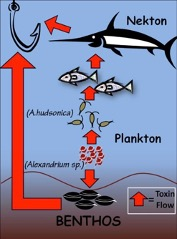
\includegraphics{images/figure1.png}
\caption{\textbf{Figure 1}. Simplified marine food web, including toxic phytoplankton}
\end{figure}

A vital link between phytoplankton and higher trophic levels is provided by copepods, a type of zooplankton. Zooplankton are animal-like plankton that need to ingest other organisms to survive. Copepods are estimated to be the most abundant animals on the planet and are the main food source for many larval fish species. This leads to the refrain: no copepods no fish.

\begin{figure}
\centering
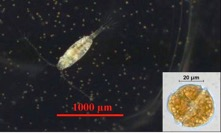
\includegraphics{images/figure2.png}
\caption{\textbf{Figure 2}. The copepod \emph{Acartia hudsonicaand} a toxic phytoplankton cell, \emph{Alexandrium fundysense}.}
\end{figure}

The toxic dinoflagellate genus \emph{Alexandrium} spp. Often blooms from Long Island Sound in the United Sates, to the Bay of Fundy, Canada (Figure 3). This bloom results in negative effects in animals (grazers) that consume it and these toxins can accumulate in the higher trophic levels, causing mortality in fish, sea birds and humans. In order to better predict the response of animal populations to the proliferation of toxic phytoplankton, \emph{Alexandrium fundysense}, scientist studied the populations of the copepod \emph{Acartia hudsonica} found in two different regions of the distribution from the Bay of Fundy, Canada, to about Long Island sound, New York and Connecticut. There are frequent and high toxicity levels in the norther region of this range (e.g., Maine) and no toxic blooms recorded in the southern regions (e.g., New Jersey).

\begin{figure}
\centering
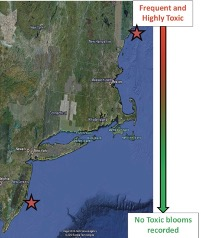
\includegraphics{images/figure3.png}
\caption{\textbf{Figure 3}. Geographical distribution of toxic \emph{Alexandrium} spp. The frequency and toxicity of \emph{Alexandrium} decreases from north to south. The copepod \emph{Acartia hudsonica}, a main grazer of toxic \emph{Alexandrium}, is found throughout the entire range shown. Stars correspond to population origins from experiments described here. Northern star indicates Maine, southern star indicates New Jersey sampling sites.}
\end{figure}

Scientist discovered that at maximum ingestion rates the Maine population had higher egg production compared to the New Jersey population (Figure 4) however when copepods were ingesting non-toxic phytoplankton there were no differences in egg production between these populations (Figure 5).

\begin{figure}
\centering
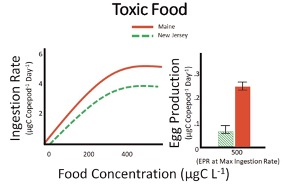
\includegraphics{images/figure4.png}
\caption{\textbf{Figure 4}. Ingestion rate (feeding; left) and egg production rate (reproduction; right) for copepods feeding on a diet containing toxic \emph{Alexandrium} spp. Ingestion rates were measured over a range of food concentrations while egg production rates correspond to a single concentration. Food saturation occurs around 500 µgCL-1; this means that this concentration represents maximum ingestion and egg production. Scientist chose this concentration for egg production because this is where the greatest difference, if any, in ingestion rate occurred. The Maine population (red) had statistically higher ingestion and egg production rate compared to copepods from New Jersey (green). Units for the dependent variable are in micrograms of carbon (µgC; food) and per copepod per day (ingestion and egg production). Error bars represent standard deviation among replicates in egg production; they are omitted for clarity from ingestion rates. Data adapted from Colin and Dam (2007, 2004).}
\end{figure}

\begin{figure}
\centering
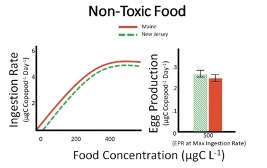
\includegraphics{images/figure5.png}
\caption{\textbf{Figure 5}. Ingestion rate (feeding; left) and egg production rate (reproduction; right) for copepods feeding on a n o-toxic diet. Ingestion rates were measured over a range of food concentrations while egg production rates correspond to a single concentration. Food saturation occurs around 500µgCL-1; this mean as that this concentration represents maximum ingestion and egg production. There were no differences between the Maine (red) and New Jersey (green) populations for both ingestion and egg production rate compared. That is, the two populations fed and reproduced at the same rate. Units and errors bars are the same as Figure 1. Data adapted from Colin and Dam (2007, 2004).}
\end{figure}

There is still much to learn about the fecundity, mortality and growth of copepods in response to toxic algae. Scientist need to better understand the interaction between toxic algae and their grazers and the adaptability of copepods to toxic algae. Understanding these relationships is key to being able to predict and mitigate issues surrounding fish populations.

\hypertarget{your-role}{%
\subsection*{Your Role}\label{your-role}}
\addcontentsline{toc}{subsection}{Your Role}

You have been hired by National Freshwater Copepod Conservation and Fish Restoration agency (NFCCFR) to investigate the impacts of toxic algae on copepod populations. The NFCCFR is interested to know what negative effects, if any, can toxic algae produce in the copepod population in freshwater populations.

Due to budget constraints you and your partner will need to conduct this research in lab and provide the NFCCFR with a proposal for approval prior to initiating your research. (The NFCCFR is your TA in case you were wondering). Before you can begin developing your proposal you must first become immersed in your topic. You and your partner will need to source out \textbf{5 primary source papers} related to this topic.

\hypertarget{macroinvertebrates-project}{%
\section*{Macroinvertebrates Project}\label{macroinvertebrates-project}}
\addcontentsline{toc}{section}{Macroinvertebrates Project}

\hypertarget{potential-changes-in-macroinvertebrates-mitigation-recommendations-needed}{%
\subsection*{Potential changes in macroinvertebrates: Mitigation recommendations needed}\label{potential-changes-in-macroinvertebrates-mitigation-recommendations-needed}}
\addcontentsline{toc}{subsection}{Potential changes in macroinvertebrates: Mitigation recommendations needed}

In Lannisport, a major town located in the city of Westeros, water sampling has been conducted by the Friends of the Turkey River Organization every three weeks from January to June in order to monitor the impacts of the Milford Farm on the Turkey River (Fig. 6).

\begin{figure}
\centering
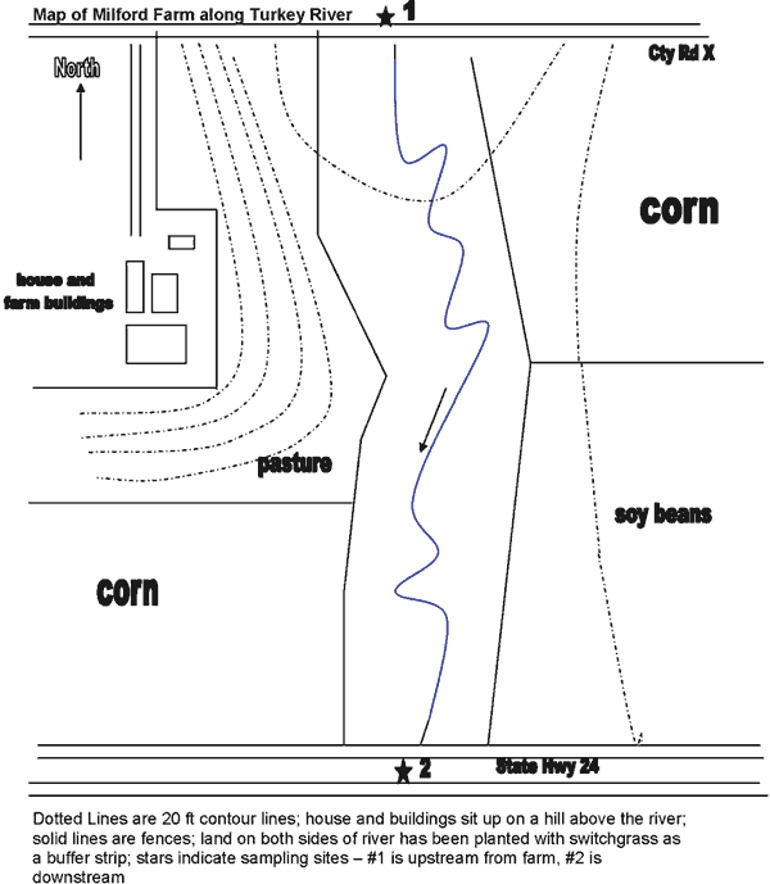
\includegraphics{images/figure6.png}
\caption{\textbf{Figure 6}. Map of Milford Farm along the Turkey River}
\end{figure}

There is growing concern that the levels in glyphosate and/or bacteria levels may impact the macroinvertebrate population found in the Turkey river. Data shown below on glyphosate levels (Fig. 2) and fecal bacterial levels (Fig. 3) have been collected every three weeks by a water quality sampling team.

\begin{figure}
\centering
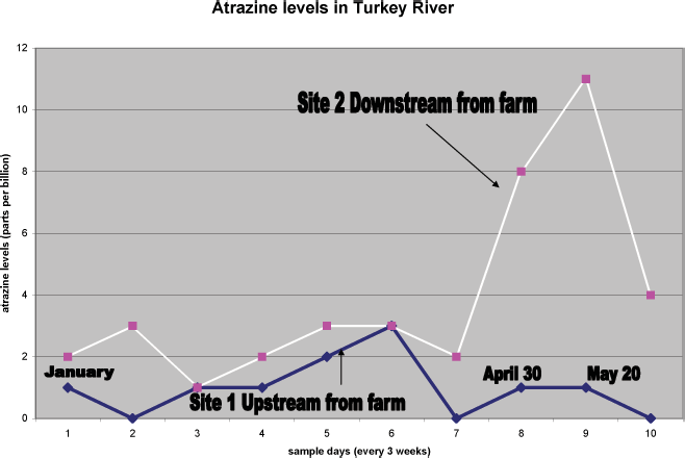
\includegraphics{images/figure7.png}
\caption{\textbf{Figure 7}. Glyphosate levels found both upstream and downstream from farm on the Milford property taken every three weeks.}
\end{figure}

\begin{figure}
\centering
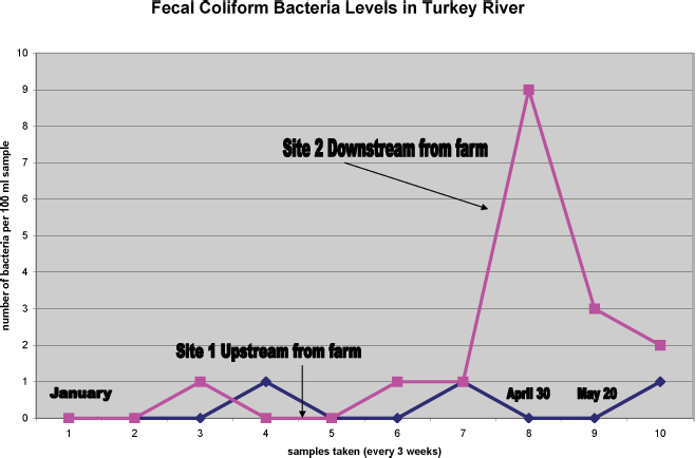
\includegraphics{images/figure8.png}
\caption{\textbf{Figure 8}. Number of fecal coliform bacterial levels per 100 ml sample upstream and downstream the farm on the Milford property taken every 3 weeks.}
\end{figure}

There is serious concern about the impacts of the farm to the water quality of the creek. The growing concern is whether or not these changes in glyphosate or bacteria levels will result in changes to the macroinvertebrate population and thus the trout population. Both macroinvertebrates and fish populations are used to assess river health however as macroinvertebrate populations are a large source for many animals in this ecological system, the Friends of the Mission Creek (FMCO) and the National Wildlife Federation (NWF) are currently interested in looking at macroinvertebrates specifically.

\hypertarget{your-role-1}{%
\subsection*{Your Role}\label{your-role-1}}
\addcontentsline{toc}{subsection}{Your Role}

You have been hired by the Friends of the Mission Creek Organization (FMCO) and the National Wildlife Federation (NWF) to investigate how this happened, what the possible effects are on the aquatic life and what can be done to prevent it from happening again.

Due to budget constraints you and your partner will need to conduct this research in lab and provide the FMCO and the NWF with a proposal for approval prior to initiating your research. (The FMCO and NWF will be represented by your TA in case you were wondering). Before you can begin developing your proposal you must first become immersed in your topic. You and your partner will need to source out \textbf{5 primary source papers} related to this topic.

\hypertarget{invasive-mussles-project}{%
\section*{Invasive Mussles Project}\label{invasive-mussles-project}}
\addcontentsline{toc}{section}{Invasive Mussles Project}

\hypertarget{invasive-mussel-project-mitigation-recommendations-needed}{%
\subsection*{Invasive Mussel Project -- Mitigation Recommendations Needed}\label{invasive-mussel-project-mitigation-recommendations-needed}}
\addcontentsline{toc}{subsection}{Invasive Mussel Project -- Mitigation Recommendations Needed}

Both the zebra and quagga mussels have been shown to be extremely destructive in the Great Lakes (NOAA, 2008). Originally from Eastern Europe they were introduced here in Canada through ballast water discharge from ships, first the zebra mussels in the 80's and then the quaggas in the 90's. As of late it appears the quagga mussels can outcompete the zebra mussels due to their ability to tolerate colder temperatures, live I soft sediment and have a much longer siphon for feeding. The NOAA's Great Lakes Environmental Research Laboratory (GLERL) have been monitoring the issue since the arrival of the quaggas. The map below (Fig. 1) illustrate how quickly the quaggas have dominated the area.

\begin{figure}
\centering
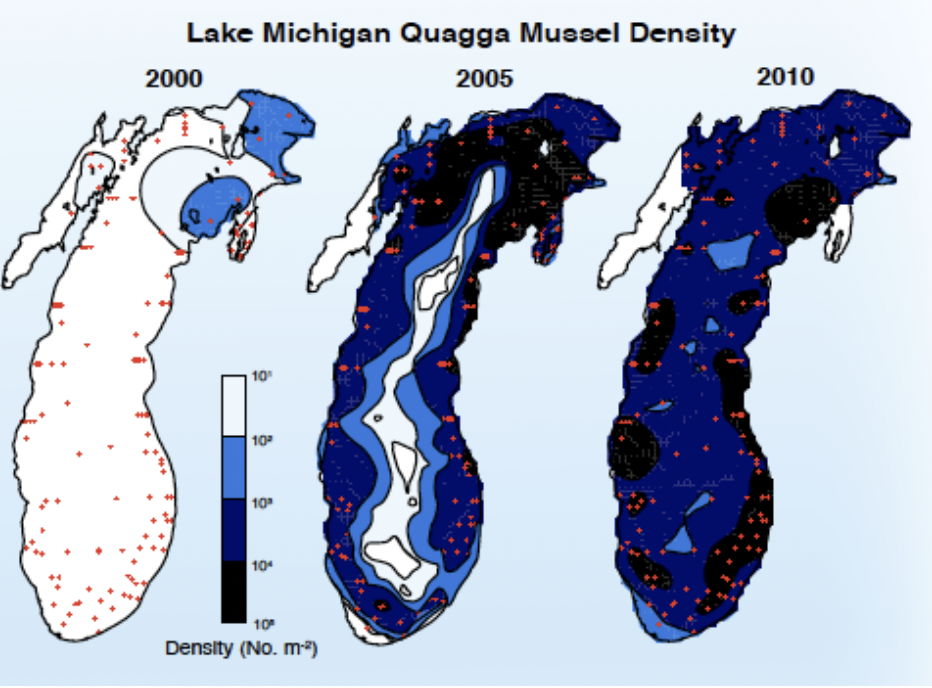
\includegraphics{images/figure9.png}
\caption{\textbf{Figure 9}. Density of Quagga Mussels in Lake Michigan determined in the year 2000, 2005 and 2010 (NOAA, 2008)}
\end{figure}

Food production for native species have been declining since the introduction of these invasive mussels and in particular the shrimp-like organisms called \emph{Diporeia} as shown in the Figure 1.

\begin{figure}
\centering
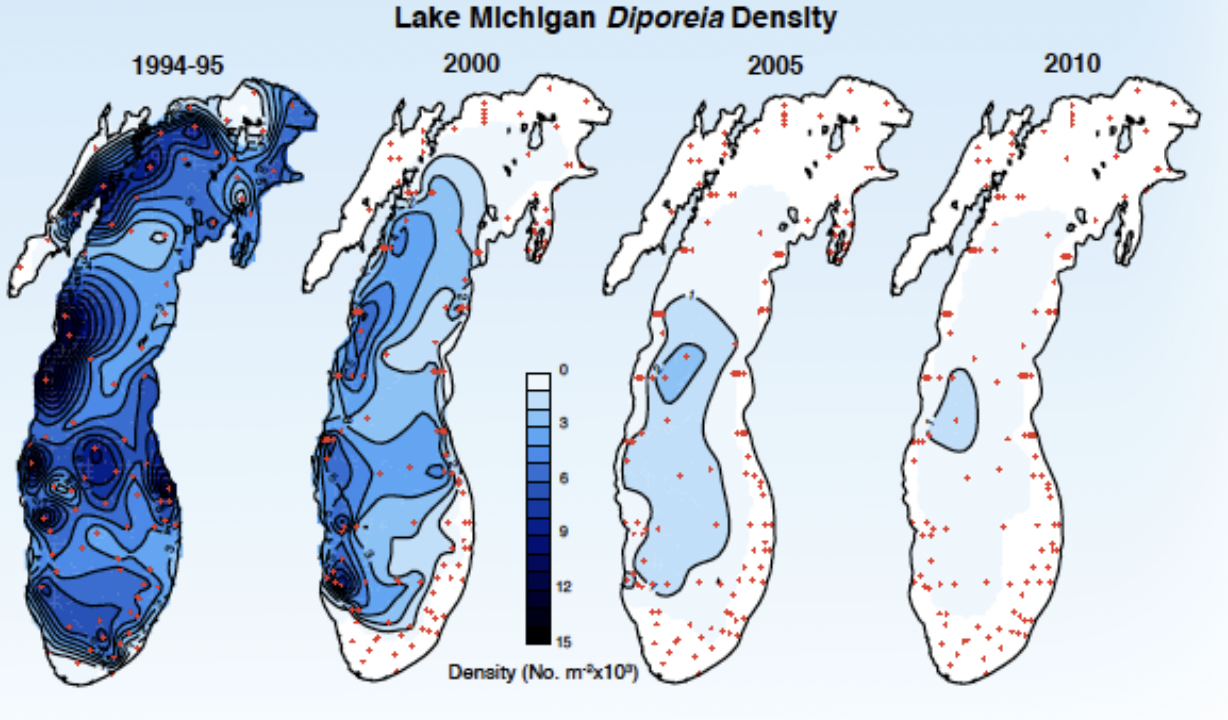
\includegraphics{images/figure10.png}
\caption{\textbf{Figure 10}. Density of \emph{Diporeia} in Lake Michigan in 1994/1995, 2000, 2005 and 2010 (NOAA, 2008)}
\end{figure}

Along with increased mussels and decreased \emph{Diporeia} researchers have seen an increase in the size and number of harmful bottom-dwelling alga in the Great Lakes. One such algal is called \emph{Cladophora}, which makes its way on to beaches in clumps rendering the beaches unpleasant due to their unsightly and smelly nature and also impact nutrient levels in the water (NOAA, 2008).

\begin{figure}
\centering
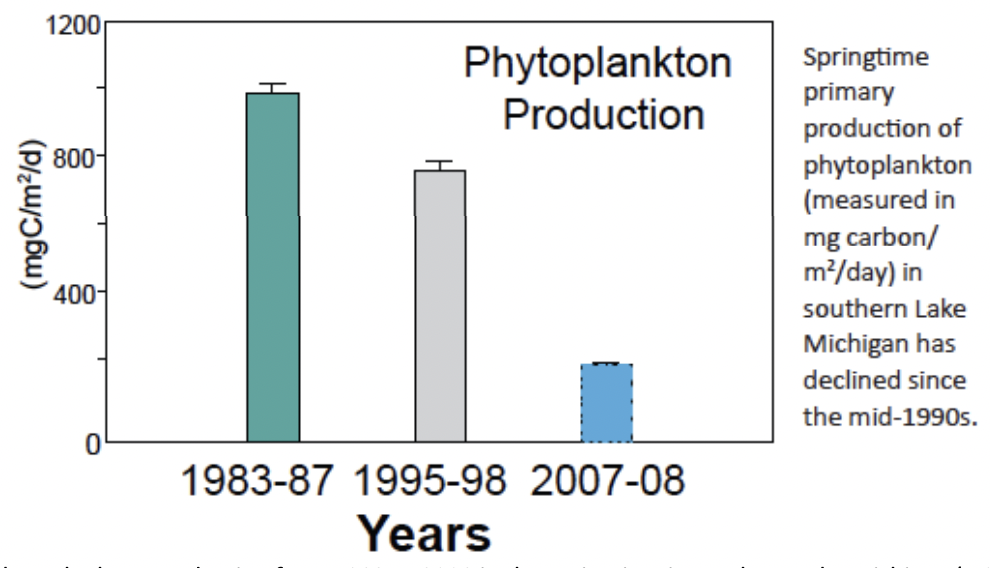
\includegraphics{images/figure11.png}
\caption{\textbf{Figure 11}. Phytoplankton production from 1983 to 2008 in the springtime in southern Lake Michigan (NOAA, 2008).)}
\end{figure}

The decline in \emph{Diporiea} has resulted in some fish changing diet to a less nutrient rich diet in order to survive. As recreational fishing has a huge presence in the Great Lakes the presence of these invasive mussels has taken its toll on the economy (NOAA, 2008). Alongside this, the tourism industry has been impacted due to the less enticing beach quality that has resulted from the \emph{Cladophoral} blooms (NOAA, 2008). Consequently, the GLERL has hired you to further investigate why and how this relationship is taking place in order to determine what mitigation strategies may be implemented.

\hypertarget{your-role-2}{%
\subsection*{Your Role}\label{your-role-2}}
\addcontentsline{toc}{subsection}{Your Role}

You have been hired by the Great Lakes Environmental Research Laboratory (GLERL) to investigate the relationship seen between invasive mussels and the harmful algal blooms. The GLERL is interested to know how these two populations are connected and what mitigation strategies can be implemented to help. Due to budget constraints you and your partner will need to conduct this research in lab and provide the GLERL with a proposal for approval prior to initiating your research. (The GLERL is your TA in case you were wondering). Before you can begin developing your proposal you must first become immersed in your topic. You and your partner will need to source out \textbf{5 primary source papers} related to this topic.

\hypertarget{part-lab-3---biol-205}{%
\part*{Lab 3 - BIOL 205}\label{part-lab-3---biol-205}}
\addcontentsline{toc}{part}{Lab 3 - BIOL 205}

\emph{Last updated 2022-09-13}

\hypertarget{getting-acquainted-with-your-organism}{%
\chapter*{Getting Acquainted with Your Organism}\label{getting-acquainted-with-your-organism}}
\addcontentsline{toc}{chapter}{Getting Acquainted with Your Organism}

As you will be working with this organism for the duration of the term it makes most sense to get to know your organism well. Thus far you have done some reading already and have likely learned a lot, however, there is nothing better than first-hand experience. This will help you in the design part of your experiment.

Based on your textbook and your previous knowledge from your primary papers research \textbf{please complete Getting Acquainted Assignment 2} on the next page.

\hypertarget{assignment-2-getting-acquainted}{%
\chapter*{Assignment 2: Getting Acquainted}\label{assignment-2-getting-acquainted}}
\addcontentsline{toc}{chapter}{Assignment 2: Getting Acquainted}

Download a copy of the assignment here. \href{https://osf.io/download/xz2rk}{BIOL205\_Assign-2\_getting-acquainted.docx}

As part of this assignment you are expected to draw a diagram of your organism. For more information on the guidelines for drawing organisms, and for some examples of poorly and properly formated sketches see \href{https://ubco-biology.github.io/Procedures-and-Guidelines/sketches-drawings.html}{Sketches \& Drawings} in the UBCO Biology Procedures and Guidelines Document.

\hypertarget{scientific-drawing-rubric}{%
\section*{Scientific Drawing Rubric}\label{scientific-drawing-rubric}}
\addcontentsline{toc}{section}{Scientific Drawing Rubric}

\textbf{Total~/18}

\begin{longtable}[]{@{}
  >{\raggedright\arraybackslash}p{(\columnwidth - 2\tabcolsep) * \real{0.5000}}
  >{\raggedright\arraybackslash}p{(\columnwidth - 2\tabcolsep) * \real{0.5000}}@{}}
\toprule()
\begin{minipage}[b]{\linewidth}\raggedright
{Criteria}
\end{minipage} & \begin{minipage}[b]{\linewidth}\raggedright
Pts
\end{minipage} \\
\midrule()
\endhead
\textbf{Caption} - No title present - Caption includes multiple sentences - Caption thoroughly described what the structure is & 3 \\
\textbf{Drawing} - Appropriate number of fine lines drawn - Dotted lines used to show depth - No shading on the drawing - Labels are organized in a column on one side of the drawing - Labels are found on the right side of the drawing - Label lines are straight - Label lines do not intersect with anything & 7 \\
\textbf{Organisms and Structures} - Drawing is oriented such that the anterior or oral aspect of organism is at the top of the page - Any structures removed or displaced have been indicated on this drawing - Genus and species are Italicized - Genus is capitalized - Specific epithet should be all lower case & 5 \\
\textbf{Microscope} - No circle is drawn around the organism - The scale (or magnification) of the drawing is at the bottom right of the drawing - Scale/magnification determination is accurate & 3 \\
\bottomrule()
\end{longtable}

\hypertarget{quiz-1-getting-acquainted}{%
\chapter*{Quiz 1: Getting Acquainted}\label{quiz-1-getting-acquainted}}
\addcontentsline{toc}{chapter}{Quiz 1: Getting Acquainted}

Complete Quiz 1: Getting Acquainted on \href{https://canvas.ubc.ca/courses/113910}{Canvas}

\hypertarget{part-lab-4---biol-205}{%
\part*{Lab 4 - BIOL 205}\label{part-lab-4---biol-205}}
\addcontentsline{toc}{part}{Lab 4 - BIOL 205}

\emph{Last updated 2022-09-13}

\hypertarget{open-science-r-rmarkdown-tutorial}{%
\chapter*{Open Science, R, \& RMarkdown Tutorial}\label{open-science-r-rmarkdown-tutorial}}
\addcontentsline{toc}{chapter}{Open Science, R, \& RMarkdown Tutorial}

You were introduced to Open Science practices, RMarkdown, and RStudio when you completed a Recommendation Report in BIOL 125. We will be using the same format and a similar template for your Registered Report in BIOL 205. However, instead of using a Shiny App to visualize your data, we'll be using R Scripts with almost all the code already written for you.

To prepare you for this, you must first review some refresher Open Science, R, \& RMarkdown tutorials, read and complete some short activities with some new material on working with the provided \texttt{R} scripts, and then complete the accompanying quiz in Canvas.

\hypertarget{overview-1}{%
\section*{Overview}\label{overview-1}}
\addcontentsline{toc}{section}{Overview}

\hypertarget{open-science}{%
\subsection*{Open Science}\label{open-science}}
\addcontentsline{toc}{subsection}{Open Science}

Open Science is a movement that tries to combat the replication crisis, questionable research practices, and flashy research trumping quality research in two ways. First, by providing different incentives and rewards for research. That is, changing what we measure as a success in research, shifting from a culture that emphasizes novel findings to one that also rewards the many other aspects of practicing good science. Second, by making all parts of the scientific research process transparent and accessible, allowing for a critical review of how a study was conducted, and ultimately enabling that study to be independently replicated.

For an optional refresher of Open Science principles and core values, visit the \href{https://ubco-biology.github.io/OS-Introduction/principles-of-open-science.html}{Open Science 101 Module} that was covered in BIOL 116.

\hypertarget{registered-reports}{%
\subsection*{Registered Reports}\label{registered-reports}}
\addcontentsline{toc}{subsection}{Registered Reports}

Writing a registered report involves submitting your research question, hypotheses, and planned methods for peer review prior to beginning data collection. Using this format enhances research quality because it gives researchers a chance alter study design and methods before investing time into data collection. Just think of a time where you spent countless hours writing an essay thinking it was perfect, only to give it to a friend to read and receive a ton of editing comments. Often readers notice things the author doesn't! Pre-registering a report also helps avoid questionable research practices like selective reporting of results and publication bias.

For your Registered Report in BIOL 205, you will follow the stages of a typical registered report and implement the following Open Science practices while working on your project:

\begin{itemize}
\tightlist
\item
  Using appropriate version control on electronic documents and proper file and data management practices throughout the experiment.

  \begin{itemize}
  \tightlist
  \item
    Be sure to follow the rules outlined in Chapters 1-5 \href{https://ubco-biology.github.io/Procedures-and-Guidelines/file-and-data-management.html}{File and Data Management} in the UBCO Biology Procedures \& Guidelines Document.
  \end{itemize}
\item
  Performing a literature review on your research topic and documenting a list of consulted studies, how they were found, and the strengths, limitations, and weaknesses of each.
\item
  Submitting a registered report draft with an established a priori hypothesis, experimental design, and plan for presenting and analyzing your data. This will be marked before the experiment implementation phase and TA feedback incorporated into the project as needed. Creating a detailed, thorough plan for your research often takes as much time as running the experiment and collecting and analyzing your data. The more you plan, including anticipating potential problems, the easier the implementation!
\item
  Implementing the study according to your plan, and noting any deviations from that plan (Note: deviations often happen, and that's OK! The key is to document them). These reflections will be submitted for marks.
\item
  Submitting and presenting a poster that details your experiences implementing the research plan (including any changes recorded, justification for changes, analysis of the data, and your interpretation and conclusion).
\end{itemize}

\hypertarget{why-use-r-rmarkdown}{%
\subsection*{Why Use R \& RMarkdown?}\label{why-use-r-rmarkdown}}
\addcontentsline{toc}{subsection}{Why Use R \& RMarkdown?}

While there are numerous programs that you can use to write lab reports, research manuscripts, and perform statistical analysis, there are so many benefits to using R \& RMarkdown!

First, R is both free and open source! Moreover, using R allows for computational reproducibility of your work. Computational reproducibility is the ability to document data and analyses so that others can understand and replicate the computations that led to the results and conclusions.

While you could use R to perform statistical analyses and write your report separately using a program like Microsoft Word. By using RMarkdown to write your lab report, you can include data analyses directly within the report which allows for everything to be stored in a single document. This makes it simple for readers to understand the computations used to conduct analyses as they read through your paper. Also, remember that there are free versions of R \& RStudio, while programs like Microsoft Word require purchased subscriptions. For your Registered Report in BIOL 205 you won't be expected to have the code for your anaylses directly embedded within your RMarkdown document but you will use pre-made R scripts to perform analyses.

\hypertarget{scientific-writing-installation-of-r-rstudio}{%
\subsection*{Scientific Writing, Installation of R \& RStudio}\label{scientific-writing-installation-of-r-rstudio}}
\addcontentsline{toc}{subsection}{Scientific Writing, Installation of R \& RStudio}

For a refresher on scientific writing, the different sections of a lab report, and setting up R \& RStudio, see the BIOL 125 Lab Manual here \url{https://ubco-biology.github.io/BIOL-125-Lab-Manual/recommendation-report.html}. \textbf{Read all of the subsections under the Recommendation Report.}

\hypertarget{assignment-template}{%
\section*{Assignment Template}\label{assignment-template}}
\addcontentsline{toc}{section}{Assignment Template}

You will use the following template for your Registered Report:

\href{https://osf.io/download/g5zxk}{20220824\_Lab03\_205\_Assignment\_V1.Rmd}

Before starting your Registered Report, we'll spend some time going through the different parts of this template.

\hypertarget{using-the-template}{%
\subsection*{Using the Template}\label{using-the-template}}
\addcontentsline{toc}{subsection}{Using the Template}

All the markdown syntax that you need for RMarkdown can be found in the \href{https://ubco-biology.github.io/Procedures-and-Guidelines/markdown-1.html}{Markdown} section of the BIOL Procedures and Guidelines.

\hypertarget{directory-structure-file-naming}{%
\subsection*{Directory Structure \& File Naming}\label{directory-structure-file-naming}}
\addcontentsline{toc}{subsection}{Directory Structure \& File Naming}

It is expected that you will have a root project folder for your work associated with this lab. And that at the minimum you will have a folder for your report, your data, your figures, and your scripts. And that you will download this template into your \texttt{report/} directory. And that lastly, you will rename the template in accordance with the file naming conventions in the \href{https://ubco-biology.github.io/Procedures-and-Guidelines/file-naming.html}{Biology Procedures and Guidelines document}.

Lastly, we'll be working with an RProject file this round to help ensure our project's working directory is properly set up in \texttt{R}.

It's important to load your project using the RProject file and not the RMarkdown file to ensure your working directory is properly set and that all the scripts and templates we'll be using work as intended!

Review the instruction \href{https://ubco-biology.github.io/Procedures-and-Guidelines/set-a-working-directory-in-rstudio.html}{here} in the Procedures and Guidelines Document, for setting up a working directory and RProject file.

Your project directory structure should look something like this once you've created your RProject file and you've downloaded a copy of the RMarkdown file:

\begin{verbatim}
├── BIOL205_RP/
│   ├── BIOL205_report.RProj
│   ├── data/
│   ├── figures/
│   ├── report/
│   │   ├── 20220101_Lab03_205_Assignment_V1.Rmd
│   ├── scripts/
\end{verbatim}

\hypertarget{yaml}{%
\subsection*{YAML}\label{yaml}}
\addcontentsline{toc}{subsection}{YAML}

The top of the template contains some front matter called YAML. YAML provides instructions to all the pieces of software involved in converting your RMarkdown document to it's outputs, in this case, \texttt{pdf}. YAML is very specific to spacing, so don't add any extra spaces!

What you need to do.

\begin{enumerate}
\def\labelenumi{\arabic{enumi}.}
\tightlist
\item
  Provide a title within the quotations after \texttt{title}.
\item
  Provide your name within the quotations after \texttt{author}.
\item
  Provide your abstract within the quotations after \texttt{abstract}.
\end{enumerate}

What might be nice to know.

\begin{enumerate}
\def\labelenumi{\arabic{enumi}.}
\tightlist
\item
  r Sys.Date() pulls the date from your computer and auto populates this for you.
\item
  The \texttt{output} tag defines the output format. Other options include \texttt{html\_document} and \texttt{word\_document}.
\end{enumerate}

What exactly is YAML?

\begin{quote}
YAML™ (rhymes with ``camel'') is a human-friendly, cross language, Unicode based data serialization language designed around the common native data types of dynamic programming languages. It is broadly useful for programming needs ranging from configuration files to internet messaging to object persistence to data auditing and visualization.
\end{quote}

Read more at \href{https://yaml.org/}{the Official YAML Web Site}

\hypertarget{document-body}{%
\subsection*{Document Body}\label{document-body}}
\addcontentsline{toc}{subsection}{Document Body}

The template is then pre-populated with first level headers for each section you're expected to include in your report. Each heading re-iterates the key elements the content of these headings should address. This is just place holder text, so replace it with your own.

\hypertarget{images-graphs}{%
\subsection*{Images \& Graphs}\label{images-graphs}}
\addcontentsline{toc}{subsection}{Images \& Graphs}

There is one sample graph referenced in the template. If you'd like to download this image and place it in your \texttt{figures/} directory to test knitting your template, the file can be downloaded \href{https://osf.io/download/nrzdu}{at this link}. And your project should look like this:

\begin{verbatim}
├── BIOL205_RP/
│   ├── BIOL205_report.RProj
│   ├── data/
│   ├── figures/
│   │   ├── MVD_BIOL125-Lab5_Fig-1-Boxplot_V1.png
│   ├── report/
│   │   ├── 20220101_Lab03_205_Assignment_V1.Rmd
│   ├── scripts/
\end{verbatim}

You might note the following directly after the image path: \texttt{\{width=50\%\}}. This reduces the image size by 50\%.

As noted in the template, you do not need to write \texttt{Figure\ 1:} before your figures; this small piece of text is handled during the conversion from RMarkdown to pdf. Any other information that you would like to include in the caption should go in the \texttt{{[}{]}} before the \texttt{()} that contain the path to the image.

Figure placement

The engine behind the conversion from RMarkdown to pdf is a typesetting application, one with pretty strict rules about how content should be formatted - much more strict than something like Microsoft Word.

What this means is that if the placement of your images will disrupt your prose - by creating large amounts of empty white space for example - this typesetting application will \emph{push} your figure to somewhere lower in your report where it won't create this white space.

Your figures should be adjacent to the relevant text in your RMarkdown file. How this manifests to your pdf might look a little different; that's ok.

\hypertarget{references}{%
\subsection*{References}\label{references}}
\addcontentsline{toc}{subsection}{References}

Just before the heading for references you'll see the following

\begin{verbatim}
\clearpage
\end{verbatim}

This creates a page break between your references section and the rest of your report.

\hypertarget{building-the-pdf}{%
\subsection*{\texorpdfstring{Building the \texttt{pdf}}{Building the pdf}}\label{building-the-pdf}}
\addcontentsline{toc}{subsection}{Building the \texttt{pdf}}

If you've installed \texttt{R}, RStudio, and the \texttt{markdown} and \texttt{tinytex} packages succesfully, when you open the template \texttt{.Rmd} file you should see an option to \texttt{Knit}.

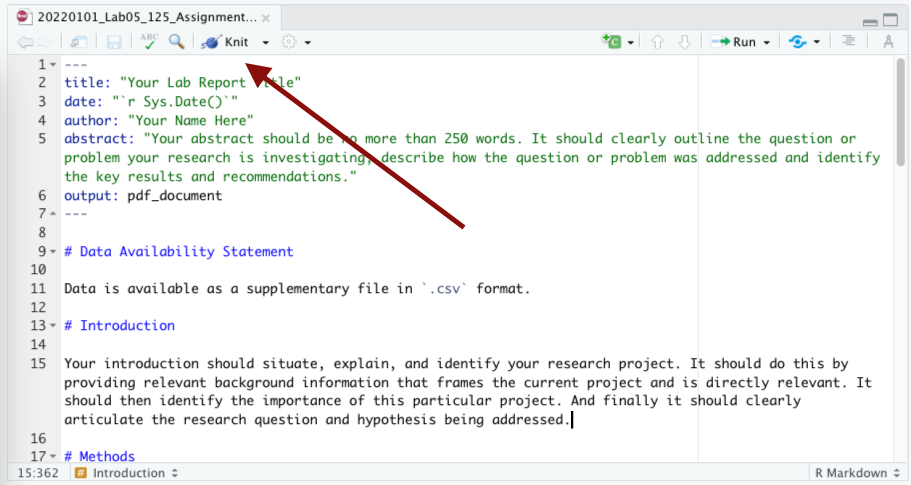
\includegraphics{images/Knit_20220101.png}

Click this button or select the drop down arrow and select \texttt{Knit\ to\ pdf}. This will generate a pdf in the same directory as your \texttt{.Rmd} file.

\hypertarget{using-the-rscripts}{%
\section*{Using the RScripts}\label{using-the-rscripts}}
\addcontentsline{toc}{section}{Using the RScripts}

Before we can knit the RMarkdown document with our own figures, we need to do our analysis and generate some visualizations! We'll do this with a few \texttt{R} scripts.

R scripts are text files containing the commands (aka code) and comments used to perform computations. For your research project, \texttt{R} scripts have been pre-written for you! You won't need to learn how to write code in \texttt{R} for this course; that comes later in BIOL 202.

There is a separate \texttt{R} script for each type of variable combination you might have for your project. Download the R script that corresponds to the types of variables you have in your experiment.

\begin{itemize}
\tightlist
\item
  Both response and explanatory variables are categorical

  \begin{itemize}
  \tightlist
  \item
    \href{https://osf.io/download/sg7y6}{BIOL205\_Script\_Categorical-Categorical.R}
  \end{itemize}
\item
  Both response and explanatory variables are quantitative

  \begin{itemize}
  \tightlist
  \item
    \href{https://osf.io/download/adwg4}{BIOL205\_Script\_Quantitative-Quantitative.R}
  \end{itemize}
\item
  Categorical explanatory variable and quantitative response variable

  \begin{itemize}
  \tightlist
  \item
    \href{https://osf.io/download/2hsk5}{BIOL205\_Script\_Quantitative-Categorical.R}
  \end{itemize}
\end{itemize}

While there are instructions within the \texttt{R} scripts themselves, the following sections describe how to use the R scripts in more detail. Be sure to read \textbf{everything here and in the R scripts!}

Alongside each line of code in the script is a comment proceeded with a hashtag (\#). The comments are either descriptions of what the code is doing or instructions describing things you need to do.

You must correctly set up your project and working directory using the instructions below for this to work. You must also not simply open your \texttt{R} script, but instead launch your RProject file and then from within R Studio load the script from the built in file manager.

The general workflow here is:

\begin{enumerate}
\def\labelenumi{\arabic{enumi}.}
\tightlist
\item
  Launch RStudio using your RPoject file
\item
  Load your data
\item
  Provide the script with your variable names and the labels you'd like to use on your graphs
\item
  Generate a graph and save it to your \texttt{figures/} directory
\item
  Run your descriptive stats and copy the relevant information to your RMarkdown file
\item
  Run you statistical analyses and copy the relevant information to your RMarkdown file
\end{enumerate}

If you quite RStudio, you will need to re-run steps 1-3 to do any of steps 4-6 again.

\hypertarget{step-1-set-your-working-directory}{%
\subsection*{Step 1: Set your working directory}\label{step-1-set-your-working-directory}}
\addcontentsline{toc}{subsection}{Step 1: Set your working directory}

If you haven't already, make sure your working directory is set according to the instructions \href{https://ubco-biology.github.io/Procedures-and-Guidelines/set-a-working-directory-in-rstudio.html}{here} in the Procedures and Guidelines Document.

Your directory should look something like this when you're done, that is, after downloading at least one script, ensuring your data is in the project's data folder, you've created an RMarkdown file, you've generated an RPoject file and put everything in its respective directory. Don't worry if you don't have all these things ready yet, just make sure that when you're ready to run your scripts with your data, this is the model you're working with.

\begin{verbatim}
├── BIOL205_RP/
│   ├── BIOL205_report.RProj
│   ├── data/
│   │   ├── 20221023_sample-data.csv
│   ├── figures/
│   ├── report/
│   │   ├── 20220101_Lab03_205_Assignment_V1.Rmd
│   ├── scripts/
│   │   ├── BIOL205_Script_Quantitative-Categorical.R
\end{verbatim}

\hypertarget{step-2-installing-loading-required-packages}{%
\subsection*{Step 2: Installing \& Loading Required Packages}\label{step-2-installing-loading-required-packages}}
\addcontentsline{toc}{subsection}{Step 2: Installing \& Loading Required Packages}

We'll be using a couple of features that are not part of the basic install of \texttt{R} in our scripts. We add additional features in \texttt{R} with packages.

Packages in \texttt{R} contain a set of functions, code, and data that you can use for your analysis. Before you can use the functions within a package, the package must be both installed in \texttt{R}, which we do once, and loaded into \texttt{R}, which we do each time we start the application.

While packages only need to be installed once, if you're on a lab computer, since the computers are re-set at the end of each day you may need to re-install packages at each log in.

To install packages noted in the \texttt{R} script, copy the installation lines of code without the preceding hashtag (\#) ie. remove the \texttt{\#} from

\begin{verbatim}
# install.packages("ggplot2")
\end{verbatim}

so it looks like this

\begin{verbatim}
install.packages("ggplot2")
\end{verbatim}

and copy it into the \texttt{R} console (lower left pane of RStudio). When you hit enter on your keyboard the package will install. Be sure to do this for all of the required packages noted in the \texttt{R} script; these are in the first few lines of each script.

Once packages are installed, they must be loaded to your current session. You will have to do this each time you re-start \texttt{R.} To load packages use the \texttt{library()} function by running the lines of code pre-written into your R script. For example, run \texttt{library(ggplot2)} by placing your cursor in that line of code and clicking the `Run' button at the top right of the working document. To load all packages at the same time, use your cursor to highlight all of the sections of code you want to run (lines 35-38 in the screenshot below), and then click `run'.

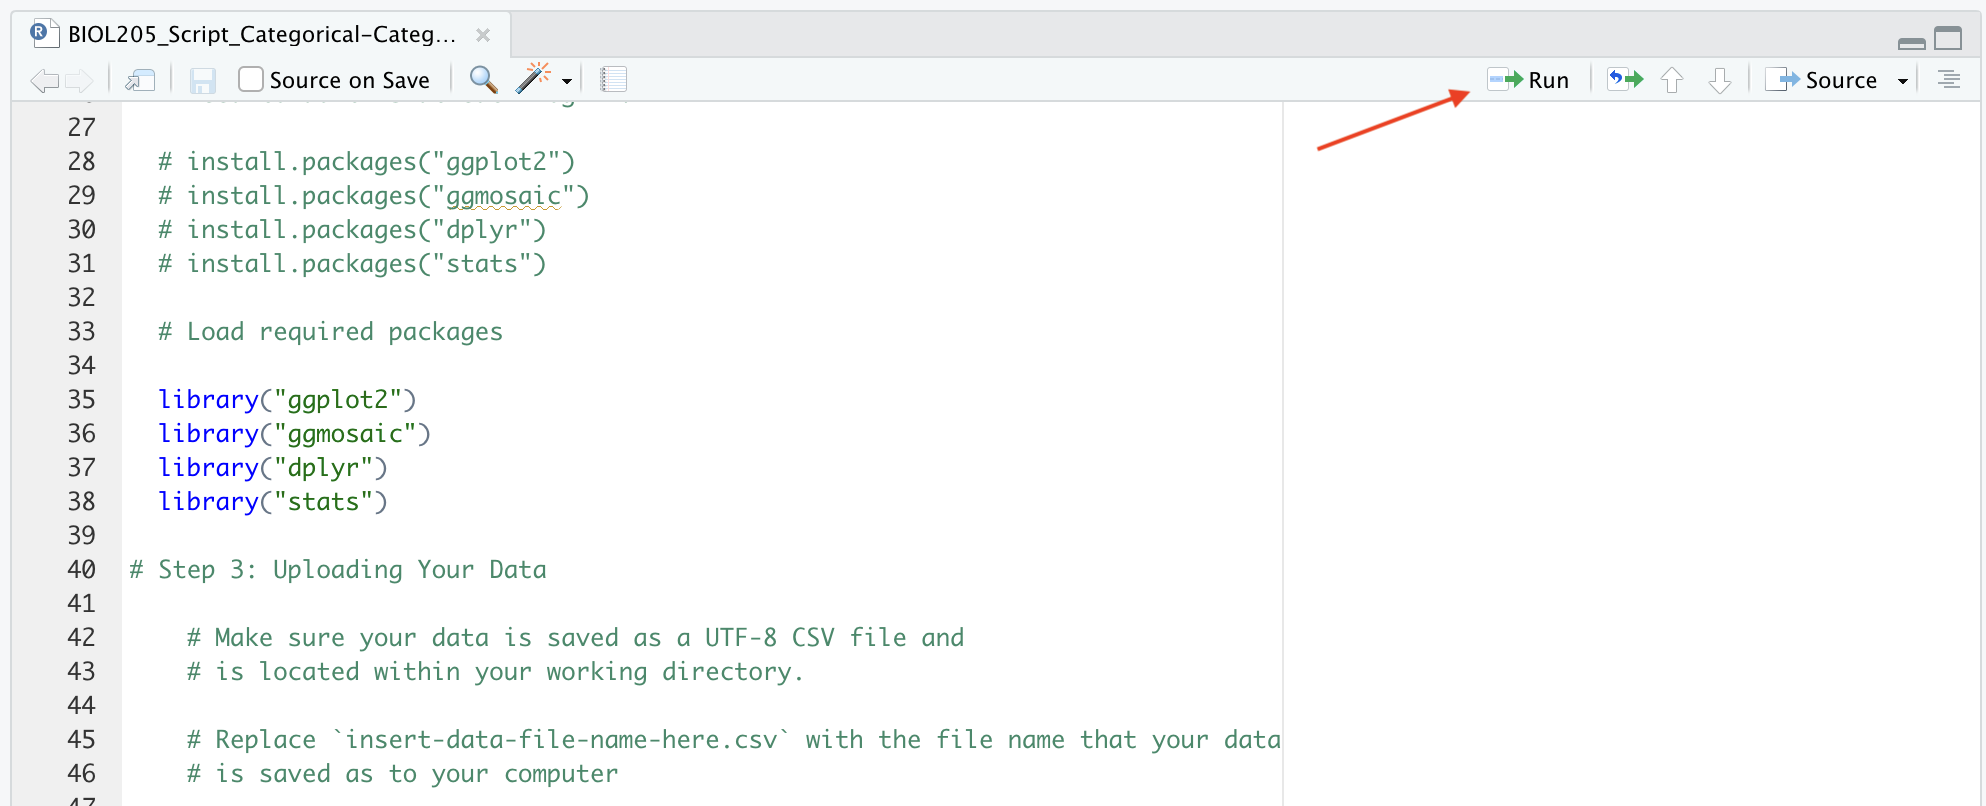
\includegraphics{images/run_button.png}

Running code can be done several ways in RStudio. You can go through line by line, putting you cursor in the line you wish to run, and executing each independently of the next. Or you can run a section of code by highlighting the `chunk' you want to run.

The scripts are broken into `steps'. It's probably best to highlight whole sections of each step and then running that chunk. But if you'd like to run line by line to get a better sense of what's happening, go for it!

To quickly run a line of code, place your cursor on the line and use \texttt{ctrl\ +\ Enter} or \texttt{Command\ +\ Enter} if you're on a Mac.

\hypertarget{step-3-uploading-your-data}{%
\subsection*{Step 3: Uploading your data}\label{step-3-uploading-your-data}}
\addcontentsline{toc}{subsection}{Step 3: Uploading your data}

Replace the content within the quotes that read `insert-data-file-name-here.csv' with the file name that your data is saved as to your computer. This will be in between lines 45 and 50 depending on the script you're using.

If my data file was called \texttt{20221023\_sample-data.csv}, I'd change the following line

\begin{verbatim}
my_file <- paste0(dir,"insert-data-file-name-here.csv") # assign file name to a variable
\end{verbatim}

to

\begin{verbatim}
my_file <- paste0(dir,"20221023_sample-data.csv") # assign file name to a variable
\end{verbatim}

If your data file contains a header row, be sure that the following line, which reads

\begin{verbatim}
my_data <- read.csv(file = my_file, header = TRUE)
\end{verbatim}

shows \texttt{header\ =\ TRUE}. If you have no header row, simply change the code to \texttt{header\ =\ FALSE}.

\hypertarget{step-4-visualizing-your-data}{%
\subsection*{Step 4: Visualizing your data}\label{step-4-visualizing-your-data}}
\addcontentsline{toc}{subsection}{Step 4: Visualizing your data}

You'll need to tell \texttt{R} some information before you can create graphs or do analyses. Specifically, you need to assign the names of your variables and axis labels. You can do this by

\begin{itemize}
\tightlist
\item
  Replacing ``X variable name'' and ``Y variable name'' with the names of your x and y variables
\item
  Replacing ``X label name'' and ``Y label name'' with your desired x and y axes labels
\end{itemize}

So, we update the following lines

\begin{verbatim}
x_var <- "X variable name" # Replace with the name of your x variable
x_label <- "X label name" # Replace with your desired x axis label
y_var <- "Y variable name" # Replace with the name of your x variable
y_label <- "Y label name" # Replace with your desired y axis label
\end{verbatim}

with something like

\begin{verbatim}
x_var <- "ht" # Replace with the name of your x variable
x_label <- "Height (in cm)" # Replace with your desired x axis label
y_var <- "day" # Replace with the name of your x variable
y_label <- "Day" # Replace with your desired y axis label
\end{verbatim}

\texttt{R} is case sensitive. When providing your variable names, make sure they match exactly the variables used in your csv file!

In the \texttt{R} script for a categorical explanatory and a categorical response variable, code for both a boxplot and a stripchart is included.

Recall that according to the \href{https://ubco-biology.github.io/Procedures-and-Guidelines/figures.html}{Biology Procedures and Guidelines document}, you should use a boxplot if the groups of your categorical variable have more than 20 data points. Alternatively, you should use a stripchart if each group contains less than 20 data points. Be sure to only produce one desired figure.

In some of the R scripts there are some additional pieces of code that you don't need to worry about for now; you'll learn more about these in BIOL 202!

For example, we have to factor the categorical variables before producing graphs. You will see this additional code if the script you are using includes categorical variables.

In the code for creating a boxplot or stripchart, we refer to a function that calculates confidence intervals. So we have to define that function prior to running the code to produce the figure. You will find this additional piece of code in your R script if your experiment has a categorical explanatory variable and quantitative response variable.

There are some regions in the R scripts where variables are re-named or manipulated. If your up for it, take some time to read through the script and see if you can figure out exactly what's happening!

Now you're ready to run the code to create your figure! Once the code has been run, your figure will show in the lower right panel of RStudio under `Plots'. To save your figure click the `Export' button and then `Save as Image'.

\hypertarget{step-5-calculate-descriptive-statistics}{%
\subsection*{Step 5: Calculate descriptive statistics}\label{step-5-calculate-descriptive-statistics}}
\addcontentsline{toc}{subsection}{Step 5: Calculate descriptive statistics}

The code here should run smoothly if everything in the proceeding steps was done correctly. Once the code has been run, your descriptive statistics will be printed in the console of RStudio (lower left panel). The instructions below describe how to interpret this output depending on the types of variables in your experiment.

\textbf{Two Categorical Variables}

Here is an example of the descriptive statistics output produced by the R script for two categorical variables. The explanatory (independent) variable and its associated groups appear in the first column, while the response (dependent) variable appears at the top. In this case the explanatory variable was species and the response variable was sex. The numbers provided in the table describe the frequency for each category. For example, in this sample there was 1 female Adelie penguin and 0 male Chinstrap penguins.

\begin{verbatim}
##            sex
## species     female male
##   Adelie        73   73
##   Chinstrap     34   34
##   Gentoo        58   61
\end{verbatim}

\textbf{Two Quantitative Variables}

Here is an example of the output produced by the R script for two quantitative variables. The explanatory (independent) variable appears in the first row, while the response (dependent) variable appears in the second row. \texttt{n} indicates the sample size, while the following columns represent the mean, standard deviation, median, and interquartile range, respectively.

\begin{verbatim}
##                  n mean   sd median  iqr
## bill_length_mm 344 43.9 5.46     NA 9.27
## bill_depth_mm  344 17.2 1.97     NA 3.10
\end{verbatim}

\textbf{One Categorical and One Quantitative Variable}

Here is an example of the output produced by the R script for one categorical and one quantitative variable. This table is organized so that the descriptive statistics of the quantitative response variable are reported based on the groups of the explanatory variable. \texttt{n} indicates the sample size, while the following columns represent the mean, standard deviation, median, and interquartile range, respectively. For example, the mean mass (g) for Adelie penguins in this sample is 3775 g.

\begin{verbatim}
##     species   n   mean     sd median   iqr
## 1    Adelie 152 3700.7 458.57   3700 650.0
## 2 Chinstrap  68 3733.1 384.34   3700 462.5
## 3    Gentoo 124 5076.0 504.12   5000 800.0
\end{verbatim}

Take a screenshot of these values or write them down for writing your lab report later.

\hypertarget{step-6-performing-statistical-analyses}{%
\subsection*{Step 6: Performing statistical analyses}\label{step-6-performing-statistical-analyses}}
\addcontentsline{toc}{subsection}{Step 6: Performing statistical analyses}

Similar to with the descriptive statistics, the code here should run smoothly if everything in the proceeding steps was done correctly. The type of statistical analyses you will perform depends on the types of variables in your experiment.

Code for all possible statistical tests is included within the R scripts. Only run the code that corresponds with the type of variables in your experiment. Use the guidelines below to help you choose the appropriate statistical test.

\textbf{Both response (dependent) and explanatory (independent) variables are categorical}

\begin{itemize}
\tightlist
\item
  Both your response and explanatory variables have exactly 2 groups -\textgreater{} Use Fisher's Exact Test
\item
  At least one of your response or explanatory variables has more than 2 groups -\textgreater{} Use Chi-Square Contingency Analysis
\end{itemize}

\textbf{Both response (dependent) and explanatory (independent) variables are quantitative}

\begin{itemize}
\tightlist
\item
  Use Correlation Analysis
\end{itemize}

\textbf{Response (dependent) variable is quantitative and explanatory (independent) variable is categorical}

\begin{itemize}
\tightlist
\item
  Your categorical variable has exactly 2 groups -\textgreater{} Use Two Sample T-test
\item
  Your categorical variable has more than 2 groups -\textgreater{} Use ANOVA
\end{itemize}

When interpreting the output from a statistical analysis for this project, focus on the p-value provided by \texttt{R.} You'll learn more about the other details shown by the output in BIOL 202! Below are some examples of output for each type of statistical test.

\textbf{Fisher's Exact Test}

\texttt{Penguins} data set with \texttt{sex} and \texttt{species} variables - the p-value is evident:

\begin{verbatim}
## 
##  Fisher's Exact Test for Count Data
## 
## data:  fisher.table
## p-value = 0.979
## alternative hypothesis: two.sided
\end{verbatim}

\textbf{Chi-Square Contingency Analysis}

\texttt{Penguins} data set with \texttt{sex} and \texttt{species} variables - the p-value is evident:

\begin{verbatim}
## 
##  Pearson's Chi-squared test
## 
## data:  chi.table
## X-squared = 0.048607, df = 2, p-value = 0.976
\end{verbatim}

\textbf{Correlation Analysis}

\texttt{Penguins} data set with \texttt{bill\_length\_mm} and \texttt{bill\_depth\_mm} variables - the p-value is fairly evident, labeled p.value:

\begin{verbatim}
## # A tibble: 1 x 8
##   estimate statistic   p.value parameter conf.low conf.high method       alter~1
##      <dbl>     <dbl>     <dbl>     <int>    <dbl>     <dbl> <chr>        <chr>  
## 1   -0.235     -4.46 0.0000112       340   -0.333    -0.132 Pearson's p~ two.si~
## # ... with abbreviated variable name 1: alternative
\end{verbatim}

\textbf{Two-Sample T-test}

\texttt{Penguins} data set with \texttt{species} - filtered to Chinstrap and Adelie - and \texttt{body\_mass\_g} variables - the p-value is evident:

\begin{verbatim}
## 
##  Two Sample t-test
## 
## data:  body_mass_g by species
## t = -0.50809, df = 217, p-value = 0.6119
## alternative hypothesis: true difference in means between group Adelie and group Chinstrap is not equal to 0
## 95 percent confidence interval:
##  -158.21193   93.35996
## sample estimates:
##    mean in group Adelie mean in group Chinstrap 
##                3700.662                3733.088
\end{verbatim}

\textbf{ANOVA}

\texttt{Penguins} data set with \texttt{species} and \texttt{body\_mass\_g} variables - the p-value is under the header Pr(\textgreater F):

\begin{verbatim}
## Analysis of Variance Table
## 
## Response: body_mass_g
##            Df    Sum Sq  Mean Sq F value    Pr(>F)    
## species     2 146864214 73432107  343.63 < 2.2e-16 ***
## Residuals 339  72443483   213698                      
## ---
## Signif. codes:  0 '***' 0.001 '**' 0.01 '*' 0.05 '.' 0.1 ' ' 1
\end{verbatim}

If you would like to have the code directly embedded within your RMarkdown report. Feel free to use the template below that corresponds with the types of variables in your research project. All of the code within these templates is the same as those described above but there are no instructions embedded in these templates.

\begin{itemize}
\tightlist
\item
  Both response and explanatory variables are categorical

  \begin{itemize}
  \tightlist
  \item
    \href{https://osf.io/download/98vmu}{20220824\_Lab03\_205\_Assignment-Categorical-Categorical\_V1.Rmd}
  \end{itemize}
\item
  Both response and explanatory variables are quantitative

  \begin{itemize}
  \tightlist
  \item
    \href{https://osf.io/download/75q4x}{20220824\_Lab03\_205\_Assignment-Quantitative-Quantitative\_V1.Rmd}
  \end{itemize}
\item
  Categorical explanatory variable and quantitative response variable

  \begin{itemize}
  \tightlist
  \item
    \href{https://osf.io/download/2hsk5}{20220824\_Lab03\_205\_Assignment-Quantitative-Categorical\_V1.Rmd}
  \end{itemize}
\end{itemize}

Similar to the R scripts, code for all possible statistical tests is included within these templates. \textbf{Only include the code that corresponds with the type of variables in your experiment.} In other words, delete the R chunk that contains code for any statistical test you are \textbf{NOT} using.

Similarly, code for both a boxplot and a stripchart is included within the quantitative-categorical template. If you plan to include a boxplot and not a stripchart, be sure to delete the R chunk that contains the code for the stripchart.

\hypertarget{quiz-2-open-science-r-rmarkdown}{%
\chapter*{Quiz 2: Open Science, R, \& RMarkdown}\label{quiz-2-open-science-r-rmarkdown}}
\addcontentsline{toc}{chapter}{Quiz 2: Open Science, R, \& RMarkdown}

Before starting this quiz, you must:

\begin{itemize}
\tightlist
\item
  practice knitting the assignment template RMarkdown file
\item
  practice using the R script for a categorical explanatory variable and quantitative response variable
\end{itemize}

\textbf{The quiz will ask you to upload a screenshots from these files and will have questions from the output of the R script!}

\hypertarget{practicing-knitting}{%
\section*{Practicing Knitting}\label{practicing-knitting}}
\addcontentsline{toc}{section}{Practicing Knitting}

If you haven't already downloaded the assignment template, here it is again:

\href{https://osf.io/download/g5zxk}{20220824\_Lab03\_205\_Assignment\_V1.Rmd}

To test the template,

\begin{itemize}
\tightlist
\item
  ensure the template \texttt{.Rmd} file is in your \texttt{report/} directory
\item
  download the following image into your \texttt{figures/} directory

  \begin{itemize}
  \tightlist
  \item
    \href{https://osf.io/download/zuehg}{MVD\_BIOL205-Lab5\_Fig-1-Boxplot\_V1.png} (4 KB)
  \end{itemize}
\item
  launch your project using your RProject file
\item
  open the template \texttt{.Rmd} file from within RStudio
\item
  insert your name as the author in the YAML header
\item
  knit the document to a PDF
\end{itemize}

You should get something that looks like this after \texttt{Knitting} the \texttt{.Rmd} file:

\begin{itemize}
\tightlist
\item
  \href{https://osf.io/download/3k8ve}{20220824\_Lab05\_125\_Assignment\_V1.pdf} (180 KB)
\end{itemize}

\textbf{Your knitted document should show your name under the title!} Take a screenshot of the first page of the knitted assignment template. You'll need to upload this screenshot to the quiz on Canvas.

\hypertarget{practicing-using-the-r-scripts}{%
\section*{Practicing Using the R Scripts}\label{practicing-using-the-r-scripts}}
\addcontentsline{toc}{section}{Practicing Using the R Scripts}

We'll practice using the R script for a categorical explanatory variable and quantitative response variable. Follow these steps:

\begin{itemize}
\tightlist
\item
  download this \texttt{R} script and save it in your \texttt{scripts/} folder

  \begin{itemize}
  \tightlist
  \item
    \href{https://osf.io/download/46mpk}{BIOL205\_Script\_Quantitative-Categorical.R}
  \end{itemize}
\item
  download this sample data set and save it in your \texttt{data/} folder

  \begin{itemize}
  \tightlist
  \item
    \href{https://osf.io/download/3r76k}{BIOL205\_sample-data.csv}
  \end{itemize}
\item
  launch your project using your RProject file
\item
  open the \texttt{R} `script from within RStudio
\item
  follow the instructions provided \href{https://ubco-biology.github.io/BIOL-205-Lab-Manual/using-the-rscripts.html}{earlier} for working with the script - setting up variable names etc - and run \emph{ALL} code in the script

  \begin{itemize}
  \tightlist
  \item
    save the boxplot produced to your \texttt{figures/} folder. You will need to upload this to the quiz on Canvas
  \item
    Keep the results of descriptive statistics and statistical analyses open while you complete the quiz. You will need some of these values to answer questions!
  \end{itemize}
\end{itemize}

\hypertarget{complete-the-quiz}{%
\section*{Complete the Quiz}\label{complete-the-quiz}}
\addcontentsline{toc}{section}{Complete the Quiz}

Now you're ready to start the quiz. Complete the Quiz titled Open Science, R, \& RMarkdown on \href{https://canvas.ubc.ca/courses/98621}{Canvas}.

\hypertarget{assignment-3-registered-report-draft}{%
\chapter*{Assignment 3: Registered Report Draft}\label{assignment-3-registered-report-draft}}
\addcontentsline{toc}{chapter}{Assignment 3: Registered Report Draft}

You will use the following template for your Registered Report:

\href{https://osf.io/download/g5zxk}{20220824\_Lab03\_205\_Assignment\_V1.Rmd} (3 KB)

See \href{https://canvas.ubc.ca}{Canvas} for assignment due dates.

For this assignment you will submit a registered report draft with an established a priori hypothesis, experimental design, and plan for presenting and analyzing your data. This will be marked before the experiment implementation phase and TA feedback incorporated into the project as needed. Creating a detailed, thorough plan for your research often takes as much time as running the experiment and collecting and analyzing your data. The more you plan, including anticipating potential problems, the easier the implementation!

At this point you won't have completed data analysis and won`'t have results to discuss. So you should focus on describing what you plan to do in detail along with explanations for why your project is importand and any potential implications results might have. For the draft research proposal you only need to include the following sections of the assignment template:

\begin{itemize}
\tightlist
\item
  Abstract
\item
  Introduction
\item
  Methods
\item
  Discussion - describe the potential implications of your project
\item
  References
\end{itemize}

When you submit the final copy of your registered report you will include \textbf{ALL} the sections of the assignment template, including the data availability statement, results etc. with a focus on your results and the direct implications and interpretaion of those specific results.

You will receive your marked Registered Report draft one week from the time it is submitted. If you have any questions regarding your mark and / or the comments from your TA please ensure you take the opportunity to chat with your TA to go over these. This will ensure that you are in the best position to attain the highest marks possible for this assignment.

\textbf{Tips for Preparing a Registered Report}

\begin{itemize}
\tightlist
\item
  Read a lot! It is important that you have a thorough understanding of the topic. At the very least you should have at least 3 primary source papers you are referring too throughout your report.
\item
  Discuss your ideas with other students (not just your partner). Get a feel for what everyone else is doing and the depth they are working in.
\item
  Start writing early! Students often make the mistake of starting the night before the report is due. This more than not results in poor submissions and thus lower grades. You should expect that you will have at least 3 rounds of revisions before you submit.
\item
  Someone reading your report should be able to tell what question(s) you will address, why the topic is interesting and/or important, how you will approach the problem, the types of data you will collect, and how your research will advance the field.
\end{itemize}

As you work on the draft of your research report, be sure to consult the Final Registered Report marking rubric \href{https://ubco-biology.github.io/BIOL-205-Lab-Manual/registered-report-rubric.html}{here}!

\hypertarget{part-lab-5---biol-205}{%
\part*{Lab 5 - BIOL 205}\label{part-lab-5---biol-205}}
\addcontentsline{toc}{part}{Lab 5 - BIOL 205}

\emph{Last updated 2022-09-13}

\hypertarget{data-collection-round-1}{%
\chapter*{Data Collection Round 1}\label{data-collection-round-1}}
\addcontentsline{toc}{chapter}{Data Collection Round 1}

This week you will be working in the labs collecting data for your project.

\hypertarget{quiz-3-who-am-i}{%
\chapter*{Quiz 3: Who Am I?}\label{quiz-3-who-am-i}}
\addcontentsline{toc}{chapter}{Quiz 3: Who Am I?}

Complete Quiz 2: Who Am I? on \href{https://canvas.ubc.ca/courses/113910}{Canvas}

\hypertarget{part-lab-6---biol-205}{%
\part*{Lab 6 - BIOL 205}\label{part-lab-6---biol-205}}
\addcontentsline{toc}{part}{Lab 6 - BIOL 205}

\emph{Last updated 2022-09-13}

\hypertarget{data-collection-round-2}{%
\chapter*{Data Collection Round 2}\label{data-collection-round-2}}
\addcontentsline{toc}{chapter}{Data Collection Round 2}

This week you will be continuing data collection for your project.

\hypertarget{assignment-4-final-registered-report}{%
\chapter*{Assignment 4: Final Registered Report}\label{assignment-4-final-registered-report}}
\addcontentsline{toc}{chapter}{Assignment 4: Final Registered Report}

\hypertarget{overview-2}{%
\section*{Overview}\label{overview-2}}
\addcontentsline{toc}{section}{Overview}

See \href{https://canvas.ubc.ca}{Canvas} for assignment due dates.

You will need to submit 4 files for this assignment:

\begin{itemize}
\tightlist
\item
  Registered report as \texttt{.Rmd}
\item
  Registered report as \texttt{.pdf}
\item
  Data in long, tidy, format as \texttt{.csv}
\item
  Data dictionary as \texttt{.md}
\end{itemize}

Following a week after you submit your Registered Report Draft you will have received the edits from your TA. You can decide to resubmit the report without making any changes or you will have the opportunity to review the edits from your TA and make the needed changes in order to increase your mark. If you have any questions regarding your mark and/or the comments from your TA please ensure you take the opportunity to chat with your TA and go over these. This will ensure that you are in the best position to attain the highest marks possible for this assignment.

When you submit the final copy of your registered report you will include \textbf{ALL} the sections of the assignment template including:

\begin{itemize}
\tightlist
\item
  Data availability statement
\item
  Introduction
\item
  Methods (including a section about statistical analyses)
\item
  Results
\item
  Discussion \& recommendations
\item
  References
\end{itemize}

\hypertarget{registered-report-rubric}{%
\section*{Registered Report Rubric}\label{registered-report-rubric}}
\addcontentsline{toc}{section}{Registered Report Rubric}

\textbf{NEEDS UPDATING}

\textbf{Total~/41}

\hypertarget{abstract}{%
\subsection*{Abstract}\label{abstract}}
\addcontentsline{toc}{subsection}{Abstract}

\textbf{~/3}

\textbf{Criteria}

\begin{itemize}
\tightlist
\item
  Brief, no more than 500 words
\item
  Clearly outlines the question/problem
\item
  Clearly describes how the question/problem will be addressed
\end{itemize}

\begin{longtable}[]{@{}
  >{\raggedright\arraybackslash}p{(\columnwidth - 2\tabcolsep) * \real{0.5000}}
  >{\raggedright\arraybackslash}p{(\columnwidth - 2\tabcolsep) * \real{0.5000}}@{}}
\toprule()
\begin{minipage}[b]{\linewidth}\raggedright
Points
\end{minipage} & \begin{minipage}[b]{\linewidth}\raggedright
{Criteria}
\end{minipage} \\
\midrule()
\endhead
Full Marks3 pts & All 3 criteria are met \\
Satisfactory2 pts & 2 of the 3 criteria are met \\
Unsatisfactory1 pt & Only 1 of the criteria is met \\
No Marks0 pts & None of the criteria are met \\
\bottomrule()
\end{longtable}

\hypertarget{introduction}{%
\subsection*{Introduction}\label{introduction}}
\addcontentsline{toc}{subsection}{Introduction}

Your Introduction \& Background should:

\begin{itemize}
\tightlist
\item
  Provide a brief literature review to contextualize the proposed research \textbf{(1-2 pages)}

  \begin{itemize}
  \tightlist
  \item
    What do you know about the organisms involved

    \begin{itemize}
    \tightlist
    \item
      What does it need to survive?
    \item
      What temperature is it typically found?
    \item
      Remember you have to run this experiment in the lab and be able to control for all variables
    \end{itemize}
  \item
    What do you know about the issue surrounding toxic algal blooms
  \item
    What differences are there between saltwater systems and freshwater systems if any that need to be considered when making inferences from one to another
  \end{itemize}
\item
  Clearly outline the problem and why this is so important. You will likely need to use the background information to justify the importance \textbf{(0.5-1 pages)}
\item
  Provide clear hypotheses
\end{itemize}

\textbf{~/6}

\textbf{Grading Criteria}

\begin{itemize}
\tightlist
\item
  Relevant background information provided
\item
  Clearly articulates how the background information is connected to the current project idea
\item
  Well written and easy to follow
\item
  Flows from more general and broad background information and narrows towards the focus of this proposed project
\item
  Hypothesis/question(s) posed are clearly stated towards the end of this section
\item
  No factual errors are present
\end{itemize}

\begin{longtable}[]{@{}
  >{\raggedright\arraybackslash}p{(\columnwidth - 2\tabcolsep) * \real{0.5000}}
  >{\raggedright\arraybackslash}p{(\columnwidth - 2\tabcolsep) * \real{0.5000}}@{}}
\toprule()
\begin{minipage}[b]{\linewidth}\raggedright
Points
\end{minipage} & \begin{minipage}[b]{\linewidth}\raggedright
{Criteria}
\end{minipage} \\
\midrule()
\endhead
Full Marks6 pts & All 6 criteria are met \\
Excellent5 pts & 5 of the 6 criteria are met \\
Proficient4 pts & 4 of the 6 criteria are met \\
Satisfactory3 pts & 3 of the 6 criteria are met \\
Unsatisfactory2 pt & 2 of the 6 criteria are met \\
Poor1 pt & Only 1 of the criteria is met \\
Incomplete0 pts & None of the criteria are met \\
\bottomrule()
\end{longtable}

\hypertarget{background}{%
\subsection*{Background}\label{background}}
\addcontentsline{toc}{subsection}{Background}

\textbf{~/4}

\textbf{Grading Criteria}

\begin{itemize}
\tightlist
\item
  Information regarding the feeding and habitat needs of the organism being used provided
\item
  The significance of using this particular organism to study the issue at hand has been provided
\item
  Information regarding the specific problem being addressed, both current and historical, have been provided
\item
  Student has shown a solid understanding of the organism, its habitat and its impact on other organisms within its range
\end{itemize}

\begin{longtable}[]{@{}
  >{\raggedright\arraybackslash}p{(\columnwidth - 2\tabcolsep) * \real{0.5000}}
  >{\raggedright\arraybackslash}p{(\columnwidth - 2\tabcolsep) * \real{0.5000}}@{}}
\toprule()
\begin{minipage}[b]{\linewidth}\raggedright
Points
\end{minipage} & \begin{minipage}[b]{\linewidth}\raggedright
{Criteria}
\end{minipage} \\
\midrule()
\endhead
Full Marks4 pts & All 4 criteria are met \\
Proficient3 pts & 3 of the 4 criteria are met \\
Satisfactory2 pts & 2 of the 4 criteria are met \\
Unsatisfactory1 pt & Only 1 of the criteria is met \\
Incomplete0 pts & None of the criteria are met \\
\bottomrule()
\end{longtable}

\hypertarget{significance-of-project}{%
\subsection*{Significance of Project}\label{significance-of-project}}
\addcontentsline{toc}{subsection}{Significance of Project}

\textbf{~/3}

\textbf{Grading Criteria}

\begin{itemize}
\tightlist
\item
  Significance of the problem is clearly and convincingly stated
\item
  Experimental design has been described in a way that elicits confidence in this study
\item
  Background information was used well in order to show the importance of this project
\end{itemize}

\begin{longtable}[]{@{}
  >{\raggedright\arraybackslash}p{(\columnwidth - 2\tabcolsep) * \real{0.5000}}
  >{\raggedright\arraybackslash}p{(\columnwidth - 2\tabcolsep) * \real{0.5000}}@{}}
\toprule()
\begin{minipage}[b]{\linewidth}\raggedright
Points
\end{minipage} & \begin{minipage}[b]{\linewidth}\raggedright
{Criteria}
\end{minipage} \\
\midrule()
\endhead
Full Marks3 pts & All 3 criteria are met \\
Satisfactory2 pts & 2 of the 3 criteria are met \\
Unsatisfactory1 pt & Only 1 of the criteria is met \\
Incomplete0 pts & None of the criteria are met \\
\bottomrule()
\end{longtable}

\hypertarget{experimental-design}{%
\subsection*{Experimental Design}\label{experimental-design}}
\addcontentsline{toc}{subsection}{Experimental Design}

Your Methods section should:

\begin{itemize}
\tightlist
\item
  Outline the major methods and data collection (including what statistical analyses to be used, when appropriate and a list of materials required). There should not be any bullet points here \textbf{(1 page)}
\end{itemize}

\textbf{~/6}

\textbf{Grading Criteria}

\begin{itemize}
\tightlist
\item
  No bullet points
\item
  The experimental design is specific and addresses the question/problem
\item
  Enough information is provided that someone else may be able to run a similar experiment
\item
  There is an appropriate control where applicable
\item
  Both independent and dependent variables are clearly defined
\item
  Statistical analysis to be used has been clearly outlined
\end{itemize}

\begin{longtable}[]{@{}
  >{\raggedright\arraybackslash}p{(\columnwidth - 2\tabcolsep) * \real{0.5000}}
  >{\raggedright\arraybackslash}p{(\columnwidth - 2\tabcolsep) * \real{0.5000}}@{}}
\toprule()
\begin{minipage}[b]{\linewidth}\raggedright
Points
\end{minipage} & \begin{minipage}[b]{\linewidth}\raggedright
{Criteria}
\end{minipage} \\
\midrule()
\endhead
Full Marks6 pts & All 6 criteria are met \\
Excellent5 pts & 5 of the 6 criteria are met \\
Proficient4 pts & 4 of the 6 criteria are met \\
Satisfactory3 pts & 3 of the 6 criteria are met \\
Unsatisfactory2 pt & 2 of the 6 criteria are met \\
Poor1 pt & Only 1 of the criteria is met \\
Incomplete0 pts & None of the criteria are met \\
\bottomrule()
\end{longtable}

\hypertarget{spelling-grammar}{%
\subsection*{Spelling \& Grammar}\label{spelling-grammar}}
\addcontentsline{toc}{subsection}{Spelling \& Grammar}

\textbf{~/3}

\textbf{Grading Criteria}

\begin{itemize}
\tightlist
\item
  No spelling errors
\item
  No grammar errors
\item
  No awkward sentence structures
\end{itemize}

\begin{longtable}[]{@{}
  >{\raggedright\arraybackslash}p{(\columnwidth - 2\tabcolsep) * \real{0.5000}}
  >{\raggedright\arraybackslash}p{(\columnwidth - 2\tabcolsep) * \real{0.5000}}@{}}
\toprule()
\begin{minipage}[b]{\linewidth}\raggedright
Points
\end{minipage} & \begin{minipage}[b]{\linewidth}\raggedright
{Criteria}
\end{minipage} \\
\midrule()
\endhead
Full Marks3 pts & All 3 criteria are met \\
Satisfactory2 pts & 2 of the 3 criteria are met \\
Unsatisfactory1 pt & Only 1 of the criteria is met \\
Incomplete0 pts & None of the criteria are met \\
\bottomrule()
\end{longtable}

\hypertarget{references-in-text-citations}{%
\subsection*{References \& In-Text Citations}\label{references-in-text-citations}}
\addcontentsline{toc}{subsection}{References \& In-Text Citations}

\textbf{~/4}

\textbf{Grading Criteria}

\begin{itemize}
\tightlist
\item
  APA format used properly and consistently
\item
  Minimum of 5 primary source papers used in the report
\item
  In-text citations are used when required
\item
  Citations and references match up
\end{itemize}

\begin{longtable}[]{@{}
  >{\raggedright\arraybackslash}p{(\columnwidth - 2\tabcolsep) * \real{0.5000}}
  >{\raggedright\arraybackslash}p{(\columnwidth - 2\tabcolsep) * \real{0.5000}}@{}}
\toprule()
\begin{minipage}[b]{\linewidth}\raggedright
Points
\end{minipage} & \begin{minipage}[b]{\linewidth}\raggedright
{Criteria}
\end{minipage} \\
\midrule()
\endhead
Full Marks4 pts & All 4 criteria are met \\
Proficient3 pts & 3 of the 4 criteria are met \\
Satisfactory2 pts & 2 of the 4 criteria are met \\
Unsatisfactory1 pt & Only 1 of the criteria is met \\
Incomplete0 pts & None of the criteria are met \\
\bottomrule()
\end{longtable}

\hypertarget{plagiarism-quotations}{%
\subsection*{Plagiarism \& Quotations}\label{plagiarism-quotations}}
\addcontentsline{toc}{subsection}{Plagiarism \& Quotations}

\textbf{~/3}

\textbf{Grading Criteria}

\begin{itemize}
\tightlist
\item
  No plagiarism of any kind has been found
\item
  No quotations present
\item
  Information attained from outside resources are properly cited
\end{itemize}

\begin{longtable}[]{@{}
  >{\raggedright\arraybackslash}p{(\columnwidth - 2\tabcolsep) * \real{0.5000}}
  >{\raggedright\arraybackslash}p{(\columnwidth - 2\tabcolsep) * \real{0.5000}}@{}}
\toprule()
\begin{minipage}[b]{\linewidth}\raggedright
Points
\end{minipage} & \begin{minipage}[b]{\linewidth}\raggedright
{Criteria}
\end{minipage} \\
\midrule()
\endhead
Full Marks3 pts & All 3 criteria are met \\
Satisfactory2 pts & 2 of the 3 criteria are met \\
Unsatisfactory1 pt & Only 1 of the criteria is met \\
Incomplete0 pts & None of the criteria are met \\
\bottomrule()
\end{longtable}

\hypertarget{format}{%
\subsection*{Format}\label{format}}
\addcontentsline{toc}{subsection}{Format}

\textbf{~/4}

\textbf{Grading Criteria}

\begin{itemize}
\tightlist
\item
  5 pages (not including references)
\item
  Font 12
\item
  Times New Roman
\item
  Double spaced
\end{itemize}

\begin{longtable}[]{@{}
  >{\raggedright\arraybackslash}p{(\columnwidth - 2\tabcolsep) * \real{0.5000}}
  >{\raggedright\arraybackslash}p{(\columnwidth - 2\tabcolsep) * \real{0.5000}}@{}}
\toprule()
\begin{minipage}[b]{\linewidth}\raggedright
Points
\end{minipage} & \begin{minipage}[b]{\linewidth}\raggedright
{Criteria}
\end{minipage} \\
\midrule()
\endhead
Full Marks4 pts & All 4 criteria are met \\
Proficient3 pts & 3 of the 4 criteria are met \\
Satisfactory2 pts & 2 of the 4 criteria are met \\
Unsatisfactory1 pt & Only 1 of the criteria is met \\
Incomplete0 pts & None of the criteria are met \\
\bottomrule()
\end{longtable}

\hypertarget{timeline}{%
\subsection*{Timeline}\label{timeline}}
\addcontentsline{toc}{subsection}{Timeline}

You must:

\begin{itemize}
\tightlist
\item
  Provide a detailed projected week by week timeline of your research. The information in this table should include the following and be in chronological order:

  \begin{itemize}
  \tightlist
  \item
    Start date of experiment (include pilot round if relevant)
  \item
    Data collection dates and how data will be collected
  \item
    Non-data collection dates should be included with a detail of what you expect to be working on. E.g. you may need to complete a water change or feed your organisms
  \item
    Additional notes may be added in the case where you anticipate there may need to be a change in timeline depending on previous weeks
  \item
    End date of experiment
  \item
    Below is an example format
  \end{itemize}
\end{itemize}

\textbf{Table 1: Projected weekly timeline}

\begin{longtable}[]{@{}
  >{\raggedright\arraybackslash}p{(\columnwidth - 4\tabcolsep) * \real{0.3333}}
  >{\raggedright\arraybackslash}p{(\columnwidth - 4\tabcolsep) * \real{0.3333}}
  >{\raggedright\arraybackslash}p{(\columnwidth - 4\tabcolsep) * \real{0.3333}}@{}}
\toprule()
\begin{minipage}[b]{\linewidth}\raggedright
Date
\end{minipage} & \begin{minipage}[b]{\linewidth}\raggedright
Activity
\end{minipage} & \begin{minipage}[b]{\linewidth}\raggedright
Notes
\end{minipage} \\
\midrule()
\endhead
\textbf{September 13, 2021} & Experimental set up - clean tank, fill with spring water and heat to appropriate temperature and add organisms & \\
\textbf{September 20th, 2021} & Count organisms using pods from a small sample and estimating total number to provide baseline population size & May need to readjust environment depending on organism survival \\
\textbf{September 27th, 2021} & Add variable - pesticides & May need to adjust amount of pesticides depending on survivability \\
\bottomrule()
\end{longtable}

\textbf{~/3}

\textbf{Grading Criteria}

\begin{itemize}
\tightlist
\item
  All data collection dates included and a description of what data will be collected and how this will be done
\item
  All non-data collection dates included with details of what will be done on those days
\item
  Start and end of dates are provided
\end{itemize}

\begin{longtable}[]{@{}
  >{\raggedright\arraybackslash}p{(\columnwidth - 2\tabcolsep) * \real{0.5000}}
  >{\raggedright\arraybackslash}p{(\columnwidth - 2\tabcolsep) * \real{0.5000}}@{}}
\toprule()
\begin{minipage}[b]{\linewidth}\raggedright
Points
\end{minipage} & \begin{minipage}[b]{\linewidth}\raggedright
{Criteria}
\end{minipage} \\
\midrule()
\endhead
Full Marks3 pts & All 3 criteria are met \\
Satisfactory2 pts & 2 of the 3 criteria are met \\
Unsatisfactory1 pt & Only 1 of the criteria is met \\
Incomplete0 pts & None of the criteria are met \\
\bottomrule()
\end{longtable}

\hypertarget{file-uploads}{%
\subsection*{File Uploads}\label{file-uploads}}
\addcontentsline{toc}{subsection}{File Uploads}

\textbf{~/2}

\textbf{Grading Criteria}

\begin{itemize}
\tightlist
\item
  Registered Report has been submitted as pdf
\item
  Registered Report has been submitted as RMarkdown
\end{itemize}

\begin{longtable}[]{@{}
  >{\raggedright\arraybackslash}p{(\columnwidth - 2\tabcolsep) * \real{0.5000}}
  >{\raggedright\arraybackslash}p{(\columnwidth - 2\tabcolsep) * \real{0.5000}}@{}}
\toprule()
\begin{minipage}[b]{\linewidth}\raggedright
Points
\end{minipage} & \begin{minipage}[b]{\linewidth}\raggedright
{Criteria}
\end{minipage} \\
\midrule()
\endhead
Full Marks2 pts & All 2 of the criteria are met \\
Unsatisfactory1 pt & Only 1 of the criteria is met \\
Incomplete0 pts & None of the criteria are met \\
\bottomrule()
\end{longtable}

\hypertarget{quiz-4-who-am-i}{%
\chapter*{Quiz 4: Who Am I?}\label{quiz-4-who-am-i}}
\addcontentsline{toc}{chapter}{Quiz 4: Who Am I?}

Complete Quiz 2: Who Am I? on \href{https://canvas.ubc.ca/courses/113910}{Canvas}

\hypertarget{part-lab-7---biol-205}{%
\part*{Lab 7 - BIOL 205}\label{part-lab-7---biol-205}}
\addcontentsline{toc}{part}{Lab 7 - BIOL 205}

\emph{Last updated 2022-09-13}

\hypertarget{data-collection-round-3}{%
\chapter*{Data Collection Round 3}\label{data-collection-round-3}}
\addcontentsline{toc}{chapter}{Data Collection Round 3}

This week you will be continuing data collection for your project.

\hypertarget{quiz-5-who-am-i}{%
\chapter*{Quiz 5: Who Am I?}\label{quiz-5-who-am-i}}
\addcontentsline{toc}{chapter}{Quiz 5: Who Am I?}

Complete Quiz 4: Who Am I? on \href{https://canvas.ubc.ca/courses/113910}{Canvas}

\hypertarget{part-lab-8---biol-205}{%
\part*{Lab 8 - BIOL 205}\label{part-lab-8---biol-205}}
\addcontentsline{toc}{part}{Lab 8 - BIOL 205}

\emph{Last updated 2022-09-13}

\hypertarget{data-collection-round-4-cleanup}{%
\chapter*{Data Collection Round 4 \& Cleanup}\label{data-collection-round-4-cleanup}}
\addcontentsline{toc}{chapter}{Data Collection Round 4 \& Cleanup}

This week you will be continuing data collection for your project.

\hypertarget{quiz-6-who-am-i}{%
\chapter*{Quiz 6: Who Am I?}\label{quiz-6-who-am-i}}
\addcontentsline{toc}{chapter}{Quiz 6: Who Am I?}

Complete Quiz 5: Who Am I? on \href{https://canvas.ubc.ca/courses/113910}{Canvas}

\hypertarget{part-lab-9---biol-205}{%
\part*{Lab 9 - BIOL 205}\label{part-lab-9---biol-205}}
\addcontentsline{toc}{part}{Lab 9 - BIOL 205}

\emph{Last updated 2022-09-13}

\hypertarget{data-analysis}{%
\chapter*{Data Analysis}\label{data-analysis}}
\addcontentsline{toc}{chapter}{Data Analysis}

For the data analysis portion of your presentation, you are permitted to use any operating program you are comfortable with. R shiny is a very simple way to run some basic stats however you are more than welcome to use R, SPSS, or even Excel depending on your needs and comfort level. Biol 202 is going to be a great resource for you so take a look through your notes. There is no assignment due for this module however you should meet with your TA online to discuss the statistical options you plan to pursue your data set and be able to explain why. This will help give your TA an opportunity to guide you and ensure you are appropriately analyzing your data in order to have the best outcome for your presentation.

R is a great way to produce your graphs however students are permitted to use whichever program they feel most comfortable using.

\hypertarget{analysis-using-r-shiny}{%
\chapter*{Analysis Using R Shiny}\label{analysis-using-r-shiny}}
\addcontentsline{toc}{chapter}{Analysis Using R Shiny}

If you are a bit uncomfortable using R, the R Shiny App is a nice way to work through your data without requiring an understanding of R.

For more information on using R Shiny please visit the following link \url{https://ubco-biology.github.io/BIOL-116-Lab-Manual/intro-to-r-shiny-apps.html}

The Shiny app you can use to run your analysis can be found here at \url{https://openscience.ok.ubc.ca/shiny/BIOL-116}

The YouTube video here can be used to walk you through the steps of using the R Shiny App 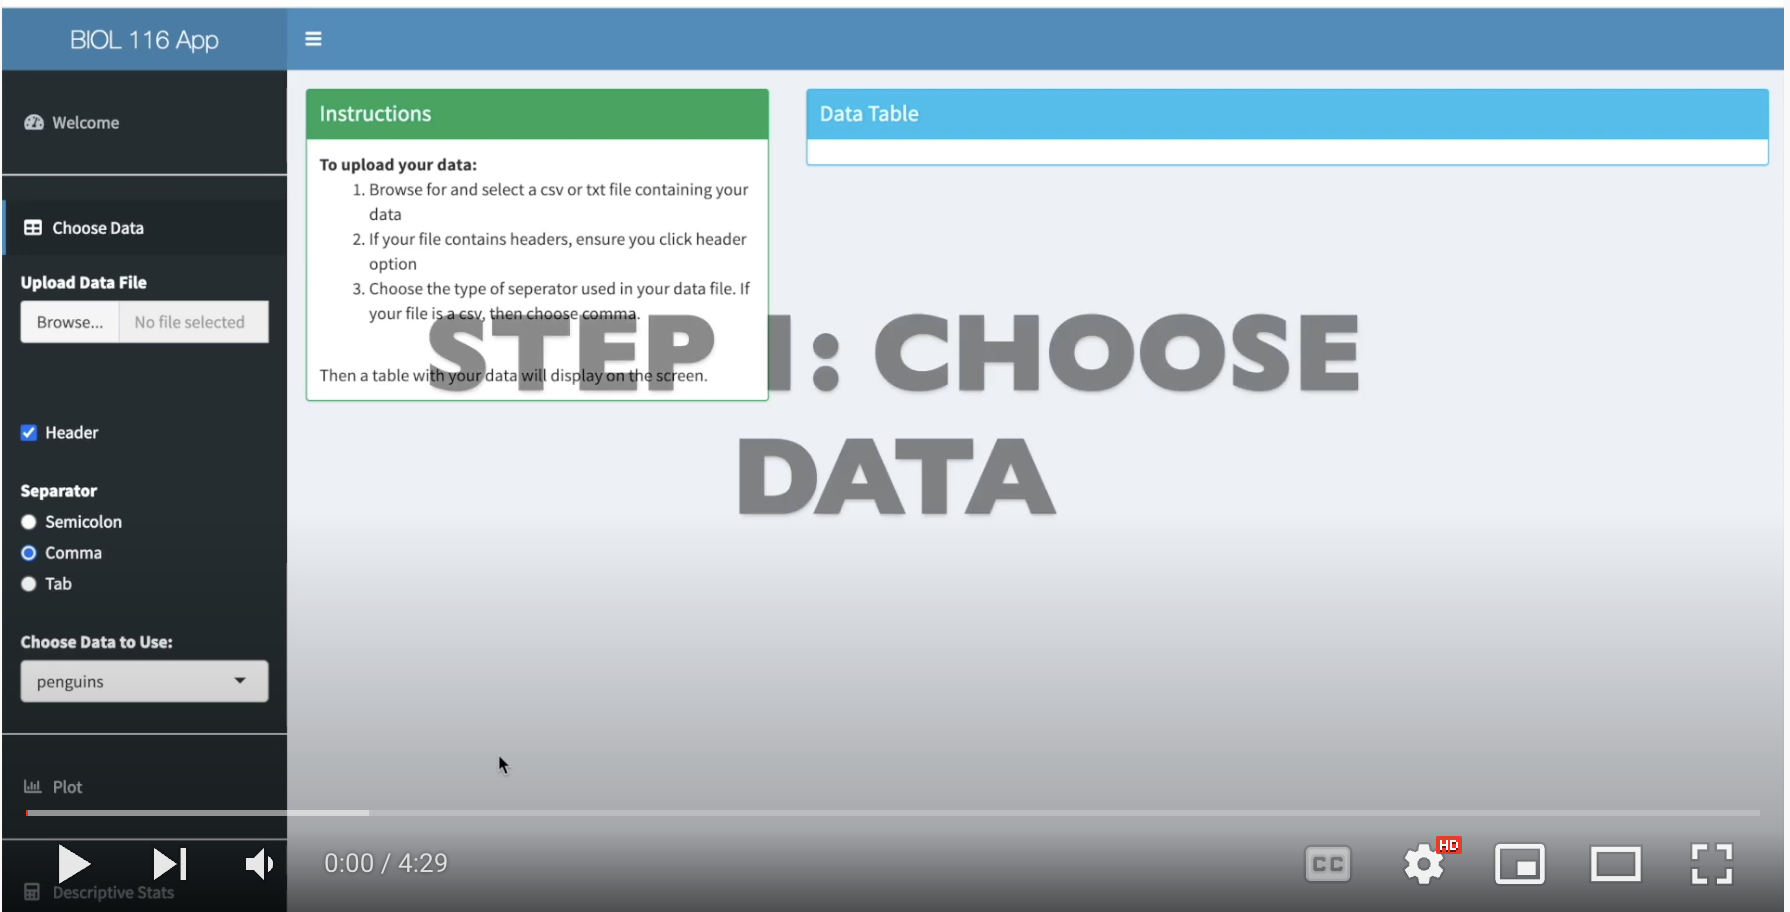
\includegraphics{images/shiny-app.png}

You may wish to refer back to the section on \href{https://ubco-biology.github.io/BIOL-116-Lab-Manual/preparing-your-data.html}{Preparing your data} from BIOL 116 and the chapter \href{https://ubco-biology.github.io/Procedures-and-Guidelines/tidy-data.html}{Tidy Data} in the UBCO Biology Procedures and Guidelines document.

\hypertarget{analysis-using-excel}{%
\chapter*{Analysis Using Excel}\label{analysis-using-excel}}
\addcontentsline{toc}{chapter}{Analysis Using Excel}

Below are a few videos which can help you get acquainted with running statistical analysis in Excel. There are much more available but this should help get you started.

\begin{itemize}
\tightlist
\item
  \href{https://www.youtube.com/watch?v=2xxMJEj4Oyg}{Basic Data Analysis in Excel - 1}
\item
  \href{https://www.youtube.com/watch?v=0wr9ojMxkuQ}{How to Perform Regression Analysis in Excel}
\item
  \href{https://www.youtube.com/watch?v=ZvfO7-J5u34}{How to Perform A One-Way ANOVA in Excel}
\item
  \href{https://www.youtube.com/watch?v=NDhmMH25AC4}{How to Perform a Chi-Square Test of Independence in Excel}
\end{itemize}

\hypertarget{part-lab-10---biol-205}{%
\part*{Lab 10 - BIOL 205}\label{part-lab-10---biol-205}}
\addcontentsline{toc}{part}{Lab 10 - BIOL 205}

\emph{Last updated 2022-09-13}

\hypertarget{assignment-5-poster-presentations}{%
\chapter*{Assignment 5: Poster Presentations}\label{assignment-5-poster-presentations}}
\addcontentsline{toc}{chapter}{Assignment 5: Poster Presentations}

\hypertarget{overview-3}{%
\section*{Overview}\label{overview-3}}
\addcontentsline{toc}{section}{Overview}

See \href{https://canvas.ubc.ca}{Canvas} for assignment due dates.

Now that you have developed a thorough understanding of the topic you will need to present your findings and provide some potential solutions to the original problem to your funders, which in this case are your peers.

All groups will give oral presentations in your regular lab period during the last week of term. Each group will have 10 minutes for their talk followed by a couple of minutes for questions. This is typically the time period allowed at a scientific conference. Each student in the group should participate equally in the presentation. Your presentation must be done using PowerPoint. A computer and projector will be available in the lab. Bring your presentation on a usb. You are also required to hand in a hard copy of your presentation at this time 24 hours prior to the start of your lab. Failure to do so will result in an instant 10\% deduction. Your group will be given a grade for the quality of your oral presentation. It is important that you;

\begin{itemize}
\tightlist
\item
  Outline your talk as early as possible
\item
  Get together to organize and practice the presentation so the timing is accurate and you do not repeat information
\item
  Remember that your goal is to present material in a clear, succinct and interesting manner.
\end{itemize}

\hypertarget{suggestions-for-content-and-structure}{%
\subsection*{Suggestions for Content and Structure}\label{suggestions-for-content-and-structure}}
\addcontentsline{toc}{subsection}{Suggestions for Content and Structure}

\begin{itemize}
\tightlist
\item
  Plan a strong, clear beginning and ending.
\item
  Provide a clear context for your work. Your introduction should include the objective and biological context of your study.
\item
  Include your hypotheses and prediction.
\item
  Present your materials and methods in a simple or streamlined manner. Keep it short and simple.
\item
  Use the PowerPoint example \href{https://osf.io/download/te4x7}{here} to help guide you
\end{itemize}

\textbf{Helpful presentation pointers for your content}

\begin{itemize}
\tightlist
\item
  Know your audience -- think about who you are presenting too. In this case you are reporting your findings to the which every organization is funding your research
\item
  Reiterate why this research was so important
\item
  Show your passion for the topic. Every story has a beginning, middle and end. For example, you started with a problem, you sought to answer it and finally you found an ``answer''.
\item
  Keep things simple! Don't make things so complicated that your audiences lose track of where you are. Keeping it simple will help everyone be able to follow along with you. When needed define abbreviated terms you plan on using. Never assume your audience will know what they mean.
\end{itemize}

\textbf{Presentation pointers for you}

\begin{itemize}
\tightlist
\item
  Practice over and over and over again until you can flow through the material without any hesitation. This will help ensure you have a handle on the material when you are nervous up at the front of the class. Take the opportunity to practice your presentation in the class
\item
  Get ready to perform. This is a performance! Know your lines and your subject. Memorizing your lines can be problematic as you may start to sound too scripted. Use bullet points to help tell you what to talk about instead. Remember you are telling a story.

  \begin{itemize}
  \tightlist
  \item
    In order to help deal with nerves before a presentation work out slowing your breathing, visualize yourself giving a relaxed talk and even tell yourself you are confident. You may even want to ``power pose'' it! For those that don't watch Grey's Anatomy this is when you stand like superman or superwomen right before attempting something that makes you nervous. There are studies indicating this is very successful but at the very least it's not going to hurt right?
  \end{itemize}
\item
  Walk confidently to the front of the room to get you in the right frame of mind
\item
  Stand tall when you are up there and keep your chest lifted. Remember you totally got this!
\item
  Above all\ldots smile! You will instantly appear more relaxed and research shows that smiling can actually reduce your stress level. Plus, there is the added benefit of people enjoying the interaction more as you don't look like you are totally miserable up there .
\item
  Speak up. People want to hear what you have to say so make sure they can.
\item
  Take your time. For you it's going to feel like its lasting forever but for your audience you may come across like you just had two coffees and a Redbull. Allow for those ``awkward'' pauses as for the audience it will actually sound more normal.
\item
  Talk to the audience and not your screen or cue cards. You should know the information so well that all you need is a quick bullet point to get you talking.
\item
  Keep to the time frame. This is where giving yourself lots of practice time will help out.
\end{itemize}

Present results clearly and simply. If you choose to present summary tables and graphs, make sure they illustrate only the points you want to make. Be sure to describe the axes before the trends in the data and ensure your figures/tables are large enough to be seen by the students at the back of the room.

Compare your results directly with the results of other similar research form the literature

Do not restrict yourselves to presenting only your best results. Mention problems you had and how you would avoid them next time as well as sources of variation and error and how these impacted your results.

\hypertarget{oral-presentation-rubric}{%
\section*{Oral Presentation Rubric}\label{oral-presentation-rubric}}
\addcontentsline{toc}{section}{Oral Presentation Rubric}

You and your partner(s) will be assessed base on the below rubric. Please use this rubric when creating and presenting your PowerPoint presentation.

\textbf{Total~/54}

\hypertarget{title-slide}{%
\subsection*{Title Slide}\label{title-slide}}
\addcontentsline{toc}{subsection}{Title Slide}

\textbf{~/3}

\textbf{Criteria}

\begin{itemize}
\tightlist
\item
  Title is clear and tells the audience what the presentation is about
\item
  All names of researchers provided
\item
  Affiliations are provided
\end{itemize}

\begin{longtable}[]{@{}
  >{\raggedright\arraybackslash}p{(\columnwidth - 2\tabcolsep) * \real{0.5000}}
  >{\raggedright\arraybackslash}p{(\columnwidth - 2\tabcolsep) * \real{0.5000}}@{}}
\toprule()
\begin{minipage}[b]{\linewidth}\raggedright
Points
\end{minipage} & \begin{minipage}[b]{\linewidth}\raggedright
{Criteria}
\end{minipage} \\
\midrule()
\endhead
Full Marks3 pts & All 3 criteria are met \\
Satisfactory2 pts & 2 of the 3 criteria are met \\
Unsatisfactory1 pt & Only 1 of the criteria is met \\
Incomplete0 pts & None of the criteria are met \\
\bottomrule()
\end{longtable}

\hypertarget{outline}{%
\subsection*{Outline}\label{outline}}
\addcontentsline{toc}{subsection}{Outline}

\textbf{~/2}

\textbf{Criteria}

\begin{itemize}
\tightlist
\item
  Outline has been provided and is clear
\item
  Outline goes over all relevant items which will be discussed
\end{itemize}

\begin{longtable}[]{@{}
  >{\raggedright\arraybackslash}p{(\columnwidth - 2\tabcolsep) * \real{0.5000}}
  >{\raggedright\arraybackslash}p{(\columnwidth - 2\tabcolsep) * \real{0.5000}}@{}}
\toprule()
\begin{minipage}[b]{\linewidth}\raggedright
Points
\end{minipage} & \begin{minipage}[b]{\linewidth}\raggedright
{Criteria}
\end{minipage} \\
\midrule()
\endhead
Full Marks2 pts & All criteria are met \\
Satisfactory1 pt & Only 1 of the criteria is met \\
Incomplete0 pts & None of the criteria are met \\
\bottomrule()
\end{longtable}

\hypertarget{background-1}{%
\subsection*{Background}\label{background-1}}
\addcontentsline{toc}{subsection}{Background}

\textbf{~/6}

\textbf{Criteria}

\begin{itemize}
\tightlist
\item
  2 slides
\item
  Only essential information has been provided
\item
  Relevancy about the project has been described
\item
  Student objectives/hypotheses have been well described
\item
  Presenter displays a clear passion for the importance of the topic and is engaging
\item
  1-2 min was provided for this section
\end{itemize}

\begin{longtable}[]{@{}
  >{\raggedright\arraybackslash}p{(\columnwidth - 2\tabcolsep) * \real{0.5000}}
  >{\raggedright\arraybackslash}p{(\columnwidth - 2\tabcolsep) * \real{0.5000}}@{}}
\toprule()
\begin{minipage}[b]{\linewidth}\raggedright
Points
\end{minipage} & \begin{minipage}[b]{\linewidth}\raggedright
{Criteria}
\end{minipage} \\
\midrule()
\endhead
Full Marks6 pts & All 6 criteria are met \\
Excellent5 pts & 5 of the 6 criteria are met \\
Proficient4 pts & 4 of the 6 criteria are met \\
Satisfactory3 pts & 3 of the 6 criteria are met \\
Unsatisfactory2 pt & 2 of the 6 criteria are met \\
Poor1 pt & Only 1 of the criteria is met \\
Incomplete0 pts & None of the criteria are met \\
\bottomrule()
\end{longtable}

\hypertarget{experimental-design-1}{%
\subsection*{Experimental Design}\label{experimental-design-1}}
\addcontentsline{toc}{subsection}{Experimental Design}

\textbf{~/6}

\textbf{Criteria}

\begin{itemize}
\tightlist
\item
  1-2 slides with
\item
  Photos/figures used help to explain the methods
\item
  Description of the design was clear with enough information provided so others can replicate
\item
  Study group is described and an explanation for why it was used is provided
\item
  Variables being tested were described
\item
  Control group described
\item
  Information regarding sample size and trial numbers was provided
\item
  Experimental design was appropriate to test the question/hypothesis
\end{itemize}

\begin{longtable}[]{@{}
  >{\raggedright\arraybackslash}p{(\columnwidth - 2\tabcolsep) * \real{0.5000}}
  >{\raggedright\arraybackslash}p{(\columnwidth - 2\tabcolsep) * \real{0.5000}}@{}}
\toprule()
\begin{minipage}[b]{\linewidth}\raggedright
Points
\end{minipage} & \begin{minipage}[b]{\linewidth}\raggedright
{Criteria}
\end{minipage} \\
\midrule()
\endhead
Full Marks6 pts & All 7 criteria are met \\
Excellent5 pts & 5-6 of the 7 criteria are met \\
Proficient4 pts & 4 of the 7 criteria are met \\
Satisfactory3 pts & 3 of the 7 criteria are met \\
Unsatisfactory2 pt & 2 of the 7 criteria are met \\
Poor1 pt & Only 1 of the criteria is met \\
Incomplete0 pts & None of the criteria are met \\
\bottomrule()
\end{longtable}

\hypertarget{results}{%
\subsection*{Results}\label{results}}
\addcontentsline{toc}{subsection}{Results}

\textbf{~/5}

\textbf{Criteria}

\begin{itemize}
\tightlist
\item
  At least 2 slides were provided which included graphs/charts etc
\item
  No raw data was provided
\item
  No figures/tables were provided and not explained
\item
  Both quantifiable and qualitative results were provided
\item
  A mixture of text, tables, figures, photos were used to convey results and those selected were the most appropriate for that type of data
\end{itemize}

\begin{longtable}[]{@{}
  >{\raggedright\arraybackslash}p{(\columnwidth - 2\tabcolsep) * \real{0.5000}}
  >{\raggedright\arraybackslash}p{(\columnwidth - 2\tabcolsep) * \real{0.5000}}@{}}
\toprule()
\begin{minipage}[b]{\linewidth}\raggedright
Points
\end{minipage} & \begin{minipage}[b]{\linewidth}\raggedright
{Criteria}
\end{minipage} \\
\midrule()
\endhead
Full Marks5 pts & All 5 criteria are met \\
Proficient4 pts & 4 of the 5 criteria are met \\
Satisfactory3 pts & 3 of the 5 criteria are met \\
Unsatisfactory2 pt & 2 of the 5 criteria are met \\
Poor1 pt & Only 1 of the criteria is met \\
Incomplete0 pts & None of the criteria are met \\
\bottomrule()
\end{longtable}

\hypertarget{discussion}{%
\subsection*{Discussion}\label{discussion}}
\addcontentsline{toc}{subsection}{Discussion}

\textbf{~/6}

\textbf{Criteria}

\begin{itemize}
\tightlist
\item
  2 slides provided
\item
  Results not repeated
\item
  Interpretation of the results was provided and was accurate
\item
  Findings were clearly presented with the most relevant to the least relevant
\item
  Results were clearly described and compared to other similar studies and their findings
\item
  Limitations to the study were clearly provided
\end{itemize}

\begin{longtable}[]{@{}
  >{\raggedright\arraybackslash}p{(\columnwidth - 2\tabcolsep) * \real{0.5000}}
  >{\raggedright\arraybackslash}p{(\columnwidth - 2\tabcolsep) * \real{0.5000}}@{}}
\toprule()
\begin{minipage}[b]{\linewidth}\raggedright
Points
\end{minipage} & \begin{minipage}[b]{\linewidth}\raggedright
{Criteria}
\end{minipage} \\
\midrule()
\endhead
Full Marks6 pts & All 6 criteria are met \\
Excellent5 pts & 5 of the 6 criteria are met \\
Good4 pts & 4 of the 6 criteria are met \\
Proficient3 pts & 3 of the 6 criteria are met \\
Satisfactory2 pt & 2 of the 6 criteria are met \\
Unsatisfactory1 pt & Only 1 of the criteria is met \\
Incomplete0 pts & None of the criteria are met \\
\bottomrule()
\end{longtable}

\hypertarget{recommendations}{%
\subsection*{Recommendations}\label{recommendations}}
\addcontentsline{toc}{subsection}{Recommendations}

\textbf{~/6}

\textbf{Criteria}

\begin{itemize}
\tightlist
\item
  Recommendations were clearly outlined
\item
  Recommendations were relevant to the problem at hand
\item
  Recommendations were based on current research
\item
  Recommendations were based on previous studies and their findings
\end{itemize}

\begin{longtable}[]{@{}ll@{}}
\toprule()
x & Points \\
\midrule()
\endhead
Full Marks6 pts & All 6 criteria are met \\
Excellent5 pts & 5 of the 6 criteria are met \\
Good4 pts & 4 of the 6 criteria are met \\
Satisfactory3 pt & 3 of the 6 criteria are met \\
Unsatisfactory2 pt & 2 of the 6 criteria are met \\
Poor1 pt & Only 1 of the criteria is met \\
Incomplete0 pts & None of the criteria are met \\
\bottomrule()
\end{longtable}

\hypertarget{acknowledgements}{%
\subsection*{Acknowledgements}\label{acknowledgements}}
\addcontentsline{toc}{subsection}{Acknowledgements}

\textbf{~/2}

\textbf{Criteria}

\begin{itemize}
\tightlist
\item
  All those individuals involved were recognized for their efforts
\item
  Funding acknowledgment was provided
\end{itemize}

\begin{longtable}[]{@{}
  >{\raggedright\arraybackslash}p{(\columnwidth - 2\tabcolsep) * \real{0.5000}}
  >{\raggedright\arraybackslash}p{(\columnwidth - 2\tabcolsep) * \real{0.5000}}@{}}
\toprule()
\begin{minipage}[b]{\linewidth}\raggedright
Points
\end{minipage} & \begin{minipage}[b]{\linewidth}\raggedright
{Criteria}
\end{minipage} \\
\midrule()
\endhead
Full Marks2 pts & All criteria are met \\
Satisfactory1 pt & Only 1 of the criteria is met \\
Incomplete0 pts & None of the criteria are met \\
\bottomrule()
\end{longtable}

\hypertarget{slide-content}{%
\subsection*{Slide Content}\label{slide-content}}
\addcontentsline{toc}{subsection}{Slide Content}

\textbf{~/5}

\textbf{Criteria}

\begin{itemize}
\tightlist
\item
  Titles for each slide told the audience exactly what they were looking at
\item
  Proper sans serif font was used
\item
  Slides were presented in the order of the outline
\item
  Slide was not wordy but rather all content is done in point form
\item
  Any copyrighted materials were cited appropriately
\end{itemize}

\begin{longtable}[]{@{}
  >{\raggedright\arraybackslash}p{(\columnwidth - 2\tabcolsep) * \real{0.5000}}
  >{\raggedright\arraybackslash}p{(\columnwidth - 2\tabcolsep) * \real{0.5000}}@{}}
\toprule()
\begin{minipage}[b]{\linewidth}\raggedright
Points
\end{minipage} & \begin{minipage}[b]{\linewidth}\raggedright
{Criteria}
\end{minipage} \\
\midrule()
\endhead
Full Marks5 pts & All 5 criteria are met \\
Proficient4 pts & 4 of the 5 criteria are met \\
Satisfactory3 pts & 3 of the 5 criteria are met \\
Unsatisfactory2 pt & 2 of the 5 criteria are met \\
Poor1 pt & Only 1 of the criteria is met \\
Incomplete0 pts & None of the criteria are met \\
\bottomrule()
\end{longtable}

\hypertarget{oral-presentation-skills}{%
\subsection*{Oral Presentation Skills}\label{oral-presentation-skills}}
\addcontentsline{toc}{subsection}{Oral Presentation Skills}

\textbf{~/7}

\textbf{Criteria}

\begin{itemize}
\tightlist
\item
  Presenters did not sound scripted
\item
  Presenters did not read of computer and/or notes
\item
  It was clear that the presenters understood the material they were presenting
\item
  Presentation fell within the appropriate time span
\item
  All charts/figures/graphs were explained thoroughly
\item
  All associations were clearly described
\item
  Questions were answered knowledgeably and professionally.
\end{itemize}

\begin{longtable}[]{@{}
  >{\raggedright\arraybackslash}p{(\columnwidth - 2\tabcolsep) * \real{0.5000}}
  >{\raggedright\arraybackslash}p{(\columnwidth - 2\tabcolsep) * \real{0.5000}}@{}}
\toprule()
\begin{minipage}[b]{\linewidth}\raggedright
Points
\end{minipage} & \begin{minipage}[b]{\linewidth}\raggedright
{Criteria}
\end{minipage} \\
\midrule()
\endhead
Full Marks7 pts & All 7 criteria are met \\
Excellent6 pts & 6 of the 7 criteria are met \\
Proficient5 pts & 5 of the 7 criteria are met \\
Satisfactory4 pts & 4 of the 7 criteria are met \\
Unsatisfactory3 pt & 3 of the 7 criteria are met \\
Insufficient2 pts & 2 of the 7 criteria are met \\
Poor1 pt & Only 1 of the criteria is met \\
Incomplete0 pts & None of the criteria are met \\
\bottomrule()
\end{longtable}

\hypertarget{additional}{%
\subsection*{Additional}\label{additional}}
\addcontentsline{toc}{subsection}{Additional}

\textbf{~/3}

\textbf{Criteria}

\begin{itemize}
\tightlist
\item
  Presentation was submitted 24 hours prior to the presentation
\item
  Each presenter contributed equally to the project
\item
  All in-text citations are references were provided
\end{itemize}

\begin{longtable}[]{@{}
  >{\raggedright\arraybackslash}p{(\columnwidth - 2\tabcolsep) * \real{0.5000}}
  >{\raggedright\arraybackslash}p{(\columnwidth - 2\tabcolsep) * \real{0.5000}}@{}}
\toprule()
\begin{minipage}[b]{\linewidth}\raggedright
Points
\end{minipage} & \begin{minipage}[b]{\linewidth}\raggedright
{Criteria}
\end{minipage} \\
\midrule()
\endhead
Full Marks3 pts & All 3 criteria are met \\
Satisfactory2 pts & 2 of the 3 criteria are met \\
Unsatisfactory1 pt & Only 1 of the criteria is met \\
Incomplete0 pts & None of the criteria are met \\
\bottomrule()
\end{longtable}

\hypertarget{slide-appearance}{%
\subsection*{Slide Appearance}\label{slide-appearance}}
\addcontentsline{toc}{subsection}{Slide Appearance}

\textbf{~/3}

\textbf{Criteria}

\begin{itemize}
\tightlist
\item
  Slides were simple, high-contrast, and had a consistent colour scheme
\item
  Slides were built to be ``colour-blind friendly''
\item
  Slides were uncluttered, clear, and visible from across the room
\end{itemize}

\begin{longtable}[]{@{}
  >{\raggedright\arraybackslash}p{(\columnwidth - 2\tabcolsep) * \real{0.5000}}
  >{\raggedright\arraybackslash}p{(\columnwidth - 2\tabcolsep) * \real{0.5000}}@{}}
\toprule()
\begin{minipage}[b]{\linewidth}\raggedright
Points
\end{minipage} & \begin{minipage}[b]{\linewidth}\raggedright
{Criteria}
\end{minipage} \\
\midrule()
\endhead
Full Marks3 pts & All 3 criteria are met \\
Satisfactory2 pts & 2 of the 3 criteria are met \\
Unsatisfactory1 pt & Only 1 of the criteria is met \\
Incomplete0 pts & None of the criteria are met \\
\bottomrule()
\end{longtable}

\end{document}
